\documentclass{imc-inf}

\title{Machine Learning and Technical Analysis for Time-series price forecasting in the financial market an empirical comparison of different approaches}
\subtitle{Sub-title of the thesis (leave empty if not required)}
\thesistype{Bachelor Thesis} % or Bachelor Expos\'e
\author{David Bobek}
\supervisor{Dipl.-Ing. Deepak Dhungana}
\copyrightyear{2023}
\submissiondate{27.11.2023}
\keywords {Machine Learning, Technical Analysis, Time-series price forecasting} 



% \usepackage{xyz}
% ... add your own packages here!
\usepackage{listings}
\usepackage{subcaption}
                              

\begin{document}
\frontmatter\maketitle{}


\begin{declarations}\end{declarations}



\begin{abstract}
	This study is going to be examining various different approaches to time-series analysis and price forecastin based on Machine Learning and Technical Analysis.
	I will be focusing on the financial market and will be trying to predict and analyse the performance of various different technical indicators and Machine learning models
	The purpose of this thesis is to compare the return and performance of my approaches and determine which of them is the most suitable for different scenarios.
	By carrying out an empirical investigation and analyzing the outcomes, I will evaluate the advantages, disadvantages and discuss potential problems.
\end{abstract}


\begin{acknowledgements}
This is an \textbf{optional} page. Use your choice of paragraph style for text on this page. Usually, this space is for thanking your supporters and getting emotional about how grateful you are to everyone.  
\end{acknowledgements}

\addtoToC{Table of Contents}%
\tableofcontents%
\clearpage


\addtoToC{List of Tables}%
\listoftables
\clearpage


\addtoToC{List of Figures}%
\listoffigures
\clearpage


%   MAIN MATTER  %%%%%%%%%%%%%%%%%%%%%%%%%%%%%%%%%%%%%%%%%%%%%%%%%%%%%%%%%%%%%%
\mainmatter%

\chapter{Introduction}\label{chap:introduction}

In today’s fast-paced capitalistically driven society in which everything is based on
planning for the future and trying to optimize the present decision, a topic of fore-
casting is well suited. In this thesis, I will be combining my passion for Data Science
and Machine Learning and will try to predict the market movement based on histor-
ically available data. Currently, there are various indicators I would like to explore
which machine learning algorithm is suited the best for which type of trend pattern
and see how my models can be used in the industry. There are several different
problems that I will be facing during this research such as Feature Selection, Over-
fitting or Generalization, or potential external factors that could affect the Financial Market.

\section{Motivation}
The goal of this thesis is to explore and help predict market trends and
eventually make their money. Trading without prior experience is difficult
and complicated. I have decided to pursue this research in order to make this
process easier. Most of the people that start trading get too scared and tend to
“FOMO” (Fear of missing out) and make incorrect decisions. I would like to there-
fore analyze and help people with this issue. By finding and recognizing different
patterns I could theoretically help spot trends and elaborate on trend patterns.
These models can also be used in the energy sector by predicting electricity or
fuel prices which can be crucial for energy companies and consumers. Machine
learning models can analyze historical data, weather patterns, and other relevant
factors to forecast energy prices accurately. This information helps energy can potentially assist companies with the optimization of production,
planning infrastructure investments, and developing pricing strategies. Machine learning models that
are based on time-series analysis and forecasting have various different use cases
and I see overall a large potential in using this technology in order to help third parties. Overall, establishing machine learning models that estimate pricing provides
useful insights to firms and individuals, allowing them to make informed decisions,
improve operations, and plan successfully in dynamic market conditions.

\section{Research Questions} 

"What is the comparative performance and predictive accuracy of a machine learning
algorithms and technical indicators for price forecasting in financial markets? The aim of this research
question is to assess a machine learning algorithm's effectiveness in price forecasting.
Through empirical investigation and analysis, I will evaluate the algorithm's advantages,
disadvantages, and practical implications in predicting financial market values for specific scenarios.


"Is it possible to predict the future price of the stock market based on historical data?" 
The aim of this research question is to assess the effectiveness of the machine learning models 
and technical indicators in predicting the future price of the stock market.
Through empirical investigation and analysis, I will evaluate the algorithm's advantages,
disadvantages, and practical implications in predicting financial market values for specific scenarios by comparing the performance of the models and indicators.



\section{Research Method} 
In my research method, I am going to create several Juptyer notebooks that will
be used to load process filter analyze and work on the data. I will be using
Python as my main programming language and will be using various different
technical indicators and machine learning models. During my research I will be  trying to find the signals that are going to be indicating the time to buy or sell 
Each of the notebooks will be focused on a different topic and will be used to display the results of my research. I will be using various different libraries such as
Pandas, Numpy, Matplotlib,Plotly, Scikit-learn, Tensorflow, Keras, Backtesting or Bokeh to make interactive visualizations and to make my research more comprehensive.



\section{State of Art}
\begin{enumerate}
	\item Gathering, analyzing and extracting important information from
	already existing sources
		\begin{itemize}
			\item  In the first step my main goal is to try to explore the thesis and information
			from elevant sources that are going to help me understand the complexity of
			this topic further. In order to stay on the correct path I will be thinking critically
			and selecting information from trusted and credited sources. My previous
			knowledge in financial markets will also be an advantage and will help me
			broaden the horizon of time-series analysis in financial markets.
		\end{itemize}

	\item Data Mining and cleaning : In order to get data of highest quality I will need
	to access it from trusted and verifiable sources. This data will most likely not
	be clean and I might need to do manual cleaning and filtering of the data.
		\begin{itemize}
			\item The second step of my approach requires collecting valuable time-series data
			of various different markets. I will be trying to mainly focus on the
			publicly traded stock market of currencies, which will be the most beneficial for me as it
			is the most traded one and its movement impacts the world the most. I am
			expecting the collected data to not be specifically ready to use and I will have
			to get rid of potential issues. For this step libraries such as Pandas and Numpy will be used.
		\end{itemize}

	\item Data Science and Analysis: This step will require a lot of Data engineering
	and digging down into what am I interested in data and which features are
	going to give us the best result based on our machine learning models and Technical Indicators
		\begin{itemize}
			\item Third step on my path will be Analyzing the data and performing an umbrella
			term called ‘Data Science’ which involves processes like data visualization,
			data exploration and statistical analysis of the data. This step will help me find
			different trend patterns in my data and further understand what is required
			from me to get better results. For this step I will be using libraries such as
			Matplotlib, Plotly, or Bokeh 
		\end{itemize}

	\item Picking the Machine Learning models and Technical Indicators. This step is going to require a lot of in-depth knwopledge 
	of the strengths and weaknesses of each Model and Indicator. Some of the models and Indicators  I could consider are 
	\begin{enumerate}
		\item Machine Learning models:
		\begin{itemize}
			\item ARIMA (Autoregressive Integrated Moving Average) models are commonly used for time
			series analysis and forecasting. They can handle both stationary and non-
			stationary time series and capture autocorrelation and offer a simple way to forecast values on a time series.
			
			\item Random Forest: Random Forest is a machine learning model that uses
			decision trees to  make predictions. It is a supervised learning algorithm that
			uses an ensemble of decision trees to make predictions. Random Forest is
			one of the most popular machine learning models for classification and could be used for time series forecasting.
			
			\item XGBoost: XGBoost is a machine learning model that also uses decision trees
			to make predictions. The difference between XGBoost and Random Forest
			is that XGBoost uses a gradient boosting algorithm to make predictions meaning that it is a boosting algorithm 
			and not an ensemble algorithm.

			\item Support Vector Regression (SVR): SVR is a machine learning model that per-
			forms regression tasks using support vector machines. By including lagged
			variables as input features, it can be modified for time series forecasting.


			\item Linear Regression: Linear Regression is the simplest machine learning model
			on this list, but in certain cases, its shear speed is unrivaled. 
			
			
	
			\item LSTM: Long Short-Term Memory (LSTM) is a type of Recurrent Neural Network
			(RNN) that can learn long-term dependencies in time series data and is therefore a good candidate for time series forecasting.
			
		\end{itemize}
		\item Technical Indicators:
		\begin{itemize}
			\item RSI (Relative Strength Index): RSI is a momentum indicator that measures the magnitude of recent price changes to evaluate overbought
			 or oversold conditions in the price of a stock or other asset.
			\item Bollinger Bands: Bollinger Bands are a technical analysis tool that measures a security's volatility and provides a relative definition 
			of high and low prices.
			\item Rolling Windows: Rolling Windows are a type of window function that computes a set of statistics for a fixed window of time and then 
			slides the window across the data by a specified interval in order to calculate the next set of statistics.
			\item Moving Averages: Moving averages is a set of lines that are used to identify trends over a certain windows when the individual moving averages are 
			crossing we can predict a trend reversal.
		\end{itemize}	
	
	 
	\end{enumerate}

		

	\item Training and Testing of Machine learning algorithms: By having high quality
	data I will be able to train the models in much fewer epochs. In this thesis I will
	be promoting less higher quality data over a lot of misleading and incorrect data. 
		\begin{itemize}
			\item Fourth step involves the actual implementation of the machine learning models based
			on training it on the train test. I am going to be experimenting with various dif-
			ferent models and training each model until I can consider its results to be
			significant enough. In this step I am also going to be implementing the Technical Indicators and combining 
			features and logic of them together in order to potentially get better results.
			The most crucial part will be the detection of the signals and updating the financial data
		accordingly to the signals For this step I will be using libraries such as 
			Scikit-learn, Tensorflow, Keras, or Backtesting

		\end{itemize}
	\item Performance Evaluation: In order to accurately evaluate my models I will be need to strategically determinge the best
	metrics to find the most optimal metric and score the models based on it. I will be using metrics such as:
	(Return on investment, Buy and hold return, Sharpe ratio, Win Trade, Accuracy, RMSE and many more)
		\begin{itemize}
		\item  The last step of my approach will be evaluating the performance of my Technical Indicators against the series of metrics 
		metrics mentioned before
		The metrics mentioned below were picked as they represent the most important aspects of the financial market and are the most important
		ones to consider when evaluating the performance of the models.
			\begin{itemize}
				\item Return on investment: Return on investment (ROI) is a financial ratio used to calculate the benefit an investor will receive in relation to their investment cost.
				 It is most commonly measured as net income divided by the original capital cost of the investment. The higher the ratio, the greater the benefit earned.
				\item Buy and hold return: Buy and hold is a passive investment strategy in which an investor buys at the current market price a financial 
				instrument and holds it for a long period of time, regardless of fluctuations in the market. An investor who uses a
				buy-and-hold strategy actively selects investments but has no concern for short-term price movements and 
				technical indicators. This metric is used to compare the performance of the models against the Technical Indicators
				\item Sharpe ratio: The Sharpe ratio is a measure of risk-adjusted return, which compares an investment's excess return to its standard deviation of returns.
				The higher the Sharpe ratio, the better the investment's historical risk-adjusted performance.
			\end{itemize}
		\item Evaluation of Metrics on the Machine Learning models is going to be different \cite{evaluation_metrics} as when using Technical Indicators. 
		While using Machine learning models I will be measuring the accuracy of the model and the RMSE (Root Mean Square Error) of the model and R2 score.
			\begin{itemize}
				\item Accuracy: Accuracy is the most obvious performance measure and it represents a ratio of correctly predicted observation to the total observations.
				What accuracy represents in time-series data is the percentage of correct predictions that the model made over time and is therefore a good metric to use when evaluating the performance of the model.
				\item RMSE: RMSE is the standard deviation of the residuals (prediction errors).
				Residuals are a measure of how far from the regression line data points are;
				RMSE is a measure of how spread out these residuals are. In other words, it tells you how concentrated the data is around the line of best fit.
				\item R2 score: R2 score is a statistical measure of how close the data are to the fitted regression line. It is also known as the coefficient of determination,
				or the coefficient of multiple determination for multiple regression.
			\end{itemize}

	
		\end{itemize}
\end{enumerate}

\section{Structure}
This thesis will be composed out of 2 parts.

	\begin{itemize}
		\item Theoretical part will be focused on
		theory and explanation of my approach and how each of the algorithms works with
		the trend pattern detection. It will require a lot of research and studying of the topic and than Mathematical
		explanation of the algorithms and their logics. The result of this part will be a sequential analysis of used Indicators and Machine Learning models.
		The second part will be a full
		\item Practical part will be focused on the implementation of the Machine Learning models and Technical Indicators.
		From data loading through data cleaning and processing to the actual implementation of the models and indicators.
		The result of this part will be a set of Juptyer notebooks that will be used to display the results of my research
		and compare the performance of the models and indicators. The technology stack I will use in this project will be
		explained in the further stages of this research. 
	\end{itemize}




\chapter{Background}\label{chap:background}

In this Chapter, we present theoretical background of related domains and technologies to set up a ground for further discussion


\section{Time series forecasting}
Time series forecasting \cite{time_ser} is a statistical technique that predicts future values or trends using past data points collected at regular intervals. It is frequently utilized in many different sectors, including finance.
Economic forecasting, weather forecasting, and sales forecasting are all examples of forecasting.
The basic premise of time series forecasting is that historical patterns and behaviors in data can provide insights into future patterns. The goal is to find underlying patterns, trends, and seasonality in time series data and utilize that knowledge to create accurate forecasts about future values.
In time series forecasting we have several topics we need to look a bit deeper into so we understand this topic more in depth.



	\begin{itemize}
		\item Stationarity
		Stationarity \cite{Smoothing_and_stationarity} is assumed for time series data, which means that its statistical features remain constant across time.
		This comprises a constant mean, constant variance, and autocovariance that is only affected by time lag.
		Many time series models rely on stationarity to produce accurate forecasts because they require steady statistical features.
		Stationarity can be spotted by comparing means and RMSE in various different places and if these 2 values do not different in many
		instances we can claim the data is stationary
		\item Smoothing
		Smoothing techniques are used to reduce noise and volatility from time series data, making underlying patterns more visible. 
		Smoothing is frequently accomplished using moving averages and exponential smoothing methods
		(such as simple exponential smoothing or double exponential smoothing). By removing noise and volatility from our data we achieve
		clearer separation in between trends allowing us to make predictions with higher accuracy This step can be compared with removing the outliers,
		however removing outliers is mostly used to delete the most extreme pieces of data. On the other hand smoothing focuses more on reducing the noises
		and is more gentle with data deletion.
		\item Seasonality Analysis
		Many time series display repeating patterns within a given time period, which is referred to as seasonality. Seasonality can occur on a daily, weekly, monthly, or other basis.
		Seasonality analysis entails detecting and modeling these periodic patterns distinct from the trend component.
		For this aim, techniques such as seasonal decomposition of time series (such as classical decomposition or STL decomposition) or Fourier analysis can be used.
		The topic of seasonality is going to be used very widely in this research as the principle of trend analysis and trend patterns work on recurring patterns and parent patterns
		(Pattern composed out of multiple patterns)

	\end{itemize}
	\section{Technical analysis}
	Technical analysis \cite{tech_analysis} is a method of evaluating financial markets that relies on the historical behavior of price.
	It is examining prior market activity and focuses on identifying patterns, support and rejection levels.
	Principle of technical analysis is to extract useful information from data and make wise decision based upon it
	Technical analysis is based on the idea that market behavior is reflecting human psychology and human emotions.
	Technical analysis takes into account emotions like fear, greed and optimism and it has deducted various different trend patterns that seem to be natural for people.
	Technical analysis also focused on the study of price charts in order to uncover repeating patterns that might assist anticipate future price changes.
	These patterns can be as simple as trend lines and support/resistance levels, or as complicated as chart patterns such as head and shoulders or triangles.
	These patterns are said to provide insights into the market's supply and demand balance as well as the psychological dynamics between buyers and sellers.
	Technical analysis is going to compose a large part of this thesis and I will be looking deeper into these patterns and trying to use data
	in which these patterns have been spotted as a traindata for my algorithms
		\subsection{Support and Resistance levels}
		Support and Resistance levels are an essential part of technical analysis and are a great indicator and insight on the current state of data.
		The principle of them is to bound already explored regions in which the trend tends to vary. This bounded zone is capped from the top by a resistance level
			\subsubsection{Support Levels}
				Support levels are levels at which demand for a security is strong enough to keep it from falling further are referred to as support levels.
				As buyers step in and produce enough demand to counteract the selling pressure, they act as a floor or "support" for the price.
				 When the price approaches a support level, it is expected to rebound and rise once more.
				Support levels can be found by looking for regions where the price has previously reversed its downward trend and begun to rise higher.
				These levels frequently correspond to prior lows or price consolidation zones on the price chart. 
				Support levels are commonly used by traders to identify potential entry points for purchasing or opening long positions
				 as there is a high probability the trend will reverse and they have a high potential of capitalizing on this
			\subsubsection{Resistance Levels}
				Resistance levels, on the other hand, are price levels at which a security's supply is sufficiently robust to prevent it from increasing higher.
				They operate as a price cap or "resistance" as sellers become more active and outnumber buyers. When the price reaches a resistance level, 
				it is expected to receive selling pressure and possibly reverse its upward trend.
				Resistance levels are identified by looking for areas where the price has previously encountered selling pressure and reversed its upward trend.
				These levels often correspond to previous highs or consolidation zones on the price chart. Traders typically use resistance levels to identify
				potential exit points for selling or taking profits from long positions.
	\section{ARIMA}

	Autoregressive moving average otherwise known as ARIMA is a Machine learning model used  for  time-series forecasting. It is used to analyze and 
	predict data points based on their temporal dependencies. It is a combination of three components: autoregression (AR), differencing (I), 
	and moving average (MA). 
	\subsection{Autoregression (AR)}
		Autoregression \cite{autoregression} is the process of modeling a variable based on its previous values. The "AR" component in ARIMA
		represents the relationship between an observation and a set number of lagged observations (i.e., the variable's historical values).
		The "p" parameter reflects the number of lag observations taken into account by the model.
		Its mathematical representation is the following:

			$AR(p): y_t = c + \phi_1 y_{t-1} + \phi_2 y_{t-2} + \ldots + \phi_p y_{t-p} + \varepsilon_t$

		Where:
			\begin{itemize}
				\item $\Delta y(t)$ represents the differenced value at time $t$.

				\item $y(t)$ denotes the original value at time $t$
				\item $y(t-1)$ represents the value at the previous time step, $t-1$.

				By applying this differencing formula to each observation in the time series, we can obtain a new series of differenced values.
				 The order of differencing refers to the number of times this process is applied. 
			\end{itemize}

		\subsection{Differencing (I)}
			Differencing is a technique that is incorporated inside of the algorithm ARIMA and its purpose is to flatten out the time series and
			 adjust it in order for it to be stationary. Stationary can be represented as low volatility of mean and variance of a specific amount of time.
			  Differencing is then useful for eliminating any patterns or seasonality. A simple formula for differencing could be represented as: 

			$\Delta y(t) = y(t) - y(t-1)$

		Where:
		\begin{itemize}
			\item $\Delta y(t)$ represents the differenced value at time $t$.
			\item $y(t)$ denotes the original value at time $t$.
			\item $y(t-l)$ represents the value at the previous time step, $t-l$.
		\end{itemize}

		\subsection{Moving Average {MA}}
			The “MA” competent is representing the dependency in between the error term at a certain time point and error time in previous time points.
			 Moving average also uses a parameter named “q”. Its sheer purpose is to represent the number of lagged terms considered in this model.
			  Mathematical formula in order to calculate the moving average for a specific time frame is:

			$y_t = c + \varepsilon_t + \theta_1 \varepsilon_{t-1} + \theta_2 \varepsilon_{t-2} + \ldots + \theta_q \varepsilon_{t-q}$

			By applying this differencing formula to each observation in the time series, we can obtain a new series of differenced values.
			 The order of differencing refers to the number of times this process is applied. 



\chapter{Related Work}\label{chap:related_work}
	In this chapter of my thesis I will be focusing on exploring and reviewing already existing academic and commercial knowledge. 
	I will be working closely with academic research and precisely studying it in order to distinguish high quality pieces of information 
	from potential false studies. There is a high potential that some pieces of academic literature might contain incorrect results as the process
	 of data preparation and cleaning could heavily skew the data towards a certain outcome and the party might not be even aware of this mistake.
	  Therefore I am going to be using only studies that seem to have a feasible approach and have not modified the outcome to fit the purpose
	   of their studies.


	\section{Academic Research}
		Machine learning is a very hot topic in the year 2023 and its combination with the well known stock market is a prevalent combination
		of the past few years. I have been able to find study such as \cite{ref1}  that have focused on in-depth analysis of performance of certain algorithms,
		however it is not directly what I will be researching . The research of deep learning algorithms used to predict the financial \cite{deep_learning}
		were very niche and well performed. I am definitely going to use the already existing findings from the author's essay in order to gain better insight
		on the current problematic of time series forecasting with deep  learning algoriths. 
		The thesis \cite{prml} has really impacted the way I started looking on this topic as it provides great results and graphs.
		The challenge it opened is to improve stock trading judgments, PRML, a revolutionary candlestick pattern recognition model based on machine learning
		methods, is proposed. To begin the pattern recognition schedule, four prominent machine learning methods and 11 different feature types are applied 
		to all potential combinations of daily patterns. To detect the prediction effect at different times, several time windows ranging from one to ten days
		are used. An investment plan is built around the recognized candlestick patterns and time span.
		The PRML model was used on the Chinese market stock for the dates  Jan 1, 2000 until Oct 30, 2020. These 20 years were splitted into training
		and testing data with a ratio 75-25 . This research was using price forecasting with multiple models including PRML. They have concluded that 
		“Empirical results show that the two-day candlestick patterns after filtering have the best prediction effect when forecasting one day ahead”
		and that applying machine learning methods to two day and three day  patterns for one day ahead forecasts can be profitable

		Possibly one of the most insightful studies is a thesis named “Machine learning techniques and data for stock market forecasting: A literature review”. \cite{lit_review} 
		Its purpose was analyzing multiple machine learning studies and conducting their results. The whole thesis was comparing the performance and quality 
		of the already existing sources. By analyzing a significant amount of studies they have been able to point out which approaches have been performing
		very well, such as: SVM (Support Vector Machine), or  ANN (Artificial neural network) \cite{Deep_learning_2} or Fuzzy Theory. These studies were conducted on different markets
		in order to diversify the machine learning models and also introduce potential differences based on geographical locations of the markets.
		This study has found out that by using neural networks on the American stock market  S\&P 500  and as input of indices data and google trends,
		they were able to achieve over 86.\% on a Hit Ratio. These results can be categorized as significant and therefore giving us a good understanding 
		on which models and approaches am I going to focus on in this thesis.



		Researchers conducting a study, \cite{arima} have conducted an in depth research on the long term performance of the already mentioned ARIMA model.
		They have been focusing on how to properly find the best fit and explained what AICc values are we looking for in order to find the model of best fit
		and then trained this model on different time series starting from 6 months and up to 23 months. They have conducted testing on 56 different stocks 
		in 6 different industries however information important are the following findings. They have achieved the highest accuracy with the model in the 
		sector Fast Moving Consumer goods of 96\% and the standard deviation of 2.03 for the 6 months. The lowest accuracy was in the banking sector with
		accuracy of 85\% and standard deviation also for the 6 months period of 15.7. This standard deviation has almost halved to 8.23 after training
		the model on 23 months of training data. They have also conducted that the p-values for all possible combinations are high, hence rejecting 
		the null hypothesis is not possible. The null hypothesis will be accepted, which is, the changes in the accuracy for different sizes of training
		datasets is not significant.

\chapter{Methodology}\label{chap:methodology}
Data collection and preparation of the data is the start of this research and I have opted to be looking at the publicly traded stock market of currencies.
My main interest is going to be the trading pair of EUR/GBP as it is among the most traded pairs in the world and its movement heavily impacts the European Market.
The goal of this research is trying to reject the null hypothesis that it is not possible to predict the future price of the stock market and capitalize on it. 

\section{Implementation}
My Implementation is going to consist of 3 main parts. Each consisting of multiple steps.
	\begin{itemize}
		\item Data Science
		\item Technical Indicators
		\item Machine Learning Models
	\end{itemize}

	\subsection{Data Science}
	In the section of data analysis I will be focusing on the analysis of the data and trying to gain information about 
	the data via visualizations and statistical analysis. I will be using libraries such as Pandas, Numpy, Matplotlib, Plotly, or Bokeh 
	in order to create visualizations and graphs that will help me understand the data better. I will be looking for patterns and analysing things as:
	When is the busiest time of the day? Does it have any effect on the price and so on.
	\begin{itemize}
		\item Data Loading: In this step I will be loading the data from the source and will be trying to get the data in the most raw form possible.
		\item Data Cleaning: In this step I will be trying to find any potential outliers or missing values and will be trying to get rid of them.
		\item  Data Analysis: In this step I will be trying to find any potential patterns and insights that could help me with the next steps.
	\end{itemize}

	\subsection{Technical Indicators}
	In this section I will be focusing on the implementation of the Technical Indicators and trying to find the best ones that will be used in the next steps.
	The Technical indicators I am going to use are for example: RSI \cite{RSI_1},Bollinger Bands \cite{Bollinger_Bands_1},Rolling Windows \cite{Rolling_window_1}, or Moving Averages \cite{Moving_average_1} and many more.
	\begin{itemize}
		\item Data Preparation: The data used to input into my Technical Indicators will be the data from the previous step and will be used to create new features.
		\item Implementation of Technical Indicators: In this step I will be implementing the Technical Indicators by at first thoroughly studying them and then extracting 
		their logic and implementing them in Python. 
		\item Signal Detection: In this step I will be capturing the signals that are going to be used in the next steps. These signals will be used to update the financial data and indicate the time to buy or sell.
		\item Evaluation of singular Indicator: This step will be focused on the evaluation of every single one of the Technical Indicators and visualising their performance.
	\end{itemize}

	\subsection{Machine Learning Models}
	In this section I will be focusing on the implementation of the Machine Learning models and trying to determine their performance and accuracy.
	The Machine Learning models I am going to use are for example: ARIMA, Random Forest, XGBoost, Support Vector Regression, Linear Regression, or LSTM.
	\begin{itemize}
		\item Data Preparation: The data used to input into my Machine Learning models will be the data from the previous steps however it wont contain the signals.
		This data will needed to be prepared in order to be used in the Machine Learning models. As we need to train the models we need to split the data into train and test data. 
		The train data will be used to train the model and the test data will be used to test the model and evaluate its performance. 
		\item Implementation of Machine Learning models: In this step I will be implementing already mentioned Machine Learning models on my time series data. 
		There is a large stigma around the Machine Learning models and their performance on time series data as this is not a common use case for them. 
		With my thesis I am trying to prove that Machine Learning models can be used for time series forecasting and can be used to predict the future price of the stock market.
		\item visualization:  In this step I will be visualizing the predictions of the Machine Learning models and comparing them with the actual price of the stock market.
		With this step I wil be able to showcase their performance and give an insight on how well they are performing.
		\item Evaluation of singular Machine Learning model: This step will be focused on the evaluation of every single one of the Machine Learning models and representing their performance. 
	\end{itemize}

	\section{Evaluation metrics}
		In this section I will be focusing on the evaluation \cite{evaluation_metrics_2} of the performance of the Machine Learning models and Technical Indicators.
		I will be using metrics such as: (Return on investment, Buy and hold return, Sharpe ratio, Win Trade, Accuracy, RMSE and many more)
		\begin{itemize}
			\item Return on investment: $ROI = \frac{Current\ Value - Original\ Value}{Original\ Value}$
			\item Buy and hold return: $Buy\ and\ hold\ return = \frac{Current\ Value - Original\ Value}{Original\ Value}$
			\item Sharpe ratio: $Sharpe\ ratio = \frac{R_p - R_f}{\sigma_p}$ => where $R_p$ is the return of the portfolio, $R_f$ is the risk-free rate of return, and $\sigma_p$ is the standard deviation of the portfolio's excess return.
			\item Win Trade: $Win\ Trade = \frac{Number\ of\ winning\ trades}{Total\ number\ of\ trades}$
			\item Accuracy: $Accuracy = \frac{Number\ of\ correct\ predictions}{Total\ number\ of\ predictions}$
			\item RMSE: $RMSE = \sqrt{\frac{\sum_{i=1}^{n} (y_i - \hat{y}_i)^2}{n}}$
			\item R2 score: $R2\ score = 1 - \frac{\sum_{i=1}^{n} (y_i - \hat{y}_i)^2}{\sum_{i=1}^{n} (y_i - \bar{y}_i)^2}$
			\item MAE: $MAE = \frac{\sum_{i=1}^{n} |y_i - \hat{y}_i|}{n}$
			\end{itemize}

		\subsection{Libraries and Technologies to be used}
			I believe it is important to mention the technologies and libraries I am going to be using in this thesis. My approach is not to reinvent the wheel and 
			use already existing data processing and visualising libraries. This will allow me to focus on the main topic of this thesis and not get distracted by
			the implementation of the libraries. I will be using the following libraries and technologies:
			\begin{itemize}
				\item Python: Python is going to be the main programming language used in this thesis. It is a very popular programming language and is used 
				heavily in the field of Data Science and Machine Learning.
				\item Jupyter Notebook: Jupyter Notebook is going to be the main IDE used in this thesis. Juptyer Notebook will allow me to create interactive
				report and visualizations that will be used to showcase the results of my research. As Juptyer Notebook allows me to run the code in blocks and store
				the results of each block it is going to be very useful for me to showcase the progress in each step of my research.
				\item Pandas: Pandas is a Python library used for data manipulation and analysis. It is used to manipulate and analyze data in a fast and efficient manner.
				\item Numpy: Numpy is a Python library used for working with arrays. It also has functions for working in domain of linear algebra, fourier transform, and matrices.
				\item  Matplotlib: Matplotlib is also a Python library used for creating static and interactive visualizations. It is a very popular library and is used in many different fields.
				For my thesis I will be using it to create visualizations of the data mainly in the form of graphs. And static analysis of the data.
				\item Plotly: Plotly is also a visualising library however it is used to create interactive visualizations. It is a very powerful library and supports a Candlestick
				charts which is going to be very useful for my thesis as almost all of my data will be in the form of Candlestick charts. (Open, High, Low, Close)
				\item Bokeh: Bokeh is also a visualising library however it is used to visualising my Backtesting results. By using Bokeh I will be able to 
				track the performance of my indicators at any given momment and see how they are performing.
				\item Scikit-learn: Scikit-learn is a Machine Learning library for Python. It is among the most popular Machine Learning libraries and
				I will be heavily using it in my thesis. It contains many different Machine Learning models such as: Random Forest, Support Vector Regression, Linear Regression and many more.
				\item Backtesting: Backtesting is a Python library used for backtesting trading strategies. It is going to be used to evaluate the performance of my Technical Indicators.
				In my thesis I will create a class for a Strategy in which I will set TP(Take Profit), SL(Stop Loss) bounderies and the strategy will be able to buy and sell at any given time.
			\end{itemize}

		\subsection{Backtesting}
			Backtesting is a process of testing a strategy\cite{what_is_backtesting} on historical data to see how it would have performed in the past. 
			This concept is often used to evaluate the effectiveness of a trading strategy and is a fairly simple process. 
			How it works step by step:
			\begin{enumerate}
				\item Starting with a set amount of capital, we buy and sell assets according to the strategy we want to test.
				\item We record the profits and losses we would have made for each trade.
				\item We repeat this process for all trades made by the strategy during the time period we are backtesting.
				\item We calculate the total profit or loss made by the strategy by adding up the profits and losses from all trades.
				\item We compare the total profit or loss to the amount of capital we started with.
			\end{enumerate}

			Backtesting as concept is also able to be represented Mathematicaly.

			\begin{itemize}
				\item The formula for calculating the total profit or loss could be represented as:
			\end{itemize}
			\begin{equation}
				\mathrm{Total Profit or Loss} = \sum_{i=1}^{n} (Sell\ Price_i - Buy\ Price_i)
			\end{equation}

			\begin{itemize}
				\item Therefore the formula for calculating the final capital could be represented as:
			\end{itemize}
			\begin{equation}
				\mathrm{Final Capital} = \mathrm{Initial Capital} + \mathrm{Total Profit or Loss}
			\end{equation}
			

\chapter{Experimentation}
	This chapter will be focused on displaying and experimenting with my proposed Technical Indicators and Machine Learning models. Each of the experimentation 
	parts will be focused on a single Technical Indicator or Machine Learning model and will be displaying its performance and accuracy. I will be following the 
	steps outlined in previous sections and will be trying to follow the same structure in order to assure a coherent structure of my research. 

	\section{Data Science}
		\subsection{Data Loading}
			The process of Data Loading is starting with finding a trust-worthy source from which I could download the data I am going to be using in my 
			research. As already mentioned  I am going to be working on the trading pair of EUR/GBP and a source from which I will be downloading the data 
			is a Swiss Banking group called Dukascopy. Dukascopy have provided me with this historical data in a form of CSV file. The data is in the form of
			Candlestick charts and contains the following columns: Date, Time, Open, High, Low, Close, Volume \cite{Technical_Indicators_with_the_Volume}. I have been able to get the data in 4 hour intervals
			which is perfect to determine the trend of the market during daily to weekly intervals. 
		\subsection{Data Cleaning}
			Data cleaning was not particularly difficult as the data was already in a very clean form. As the data provided by Dukascopy was a global data which is 
			traceable backwards it did not contain any missing values. Also in terms of outliers there is no such a concept in the stock market as the price of the 
			market is always changing and there is no such a thing as a price that is too high or too low. The only thing that could be considered as an outlier is 
			an incorrect value that the data provider could have secretly added to the data. However this is not the case and the data is very clean and almost ready to be used.
			The only thing that had to be done is renaming the column values as there was an initial issue which caused problems
		\subsection{Data Analysis}
			
			I have created a separate Juptyer Notebook called: $volume_time_analysis.ipynb$ that contains an analysis of what is the busiest hour during the day and what is the busiest hour during the 
			day and if it somewhow correlates with the price of the stock market. I have been able to find out that the busiest hour during the day and by the 
			chart we can see that the busiest hours are: 11:00 and 15:00. (GMT+2) This is a very interesting finding and also very reasonable as these are the times 
			when London Stock Exchange opens and closes.
			\begin{figure}[h!]
				\centering
				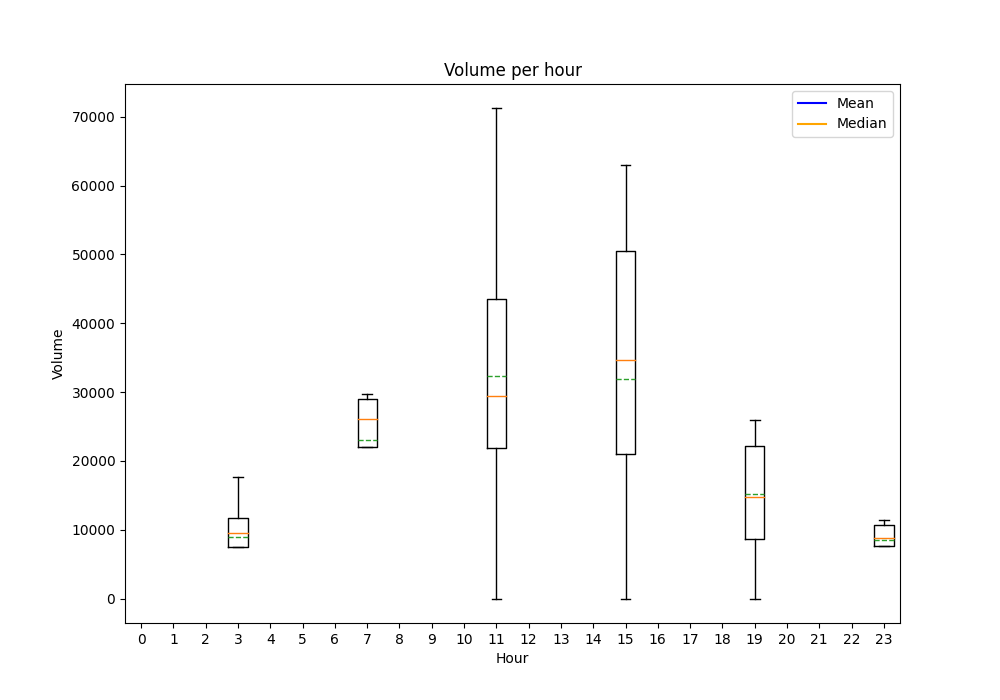
\includegraphics[width=0.8\textwidth]{volumte_time_analysis_histogram.png}
				\caption{Volume Time Analysis}
				\label{fig:volume_time_analysis}
			\end{figure} The London Stock Exchange is the largest stock exchange in Europe and the 3rd largest in the world.
			Its opening and closing times are 8:00 - 16:30 (GMT+1) and therefore the busiest hours are 11:00 and 15:00 (GMT+2). Its sheer impact on the stock market can easily move the 
			price of the pair (EURGBP). Hedge funds and other large financial institutions are also very active during these hours and therefore it is very reasonable to see this high trading volume 
			during these hours. High volume of trading can change the price however if we have the same amount of buys than sells the price will not be going one way. The market needs to make 
			an "internal agreement" in order to determine the direction it is going to be heading.
			
			This theory can also be seen on the actual line chart of how the price moves during the day. 
			The second figure in this section is showing the line chart with each distinct hour highlighted with a different color in order 
			to see the differences. This plots tracks 100 hours worth of trading as the interval in between each of the points is 4 hours and there are 25 points in total.
			I have decided to only display a fraction of the entire data due to the fact I wanted to display the differences in between the hours and not the market movement itself.
			This way we can clearly see the integer values of each of the hours and how the price is moving during these hours.
			\begin{figure}[!h!]
				\centering
				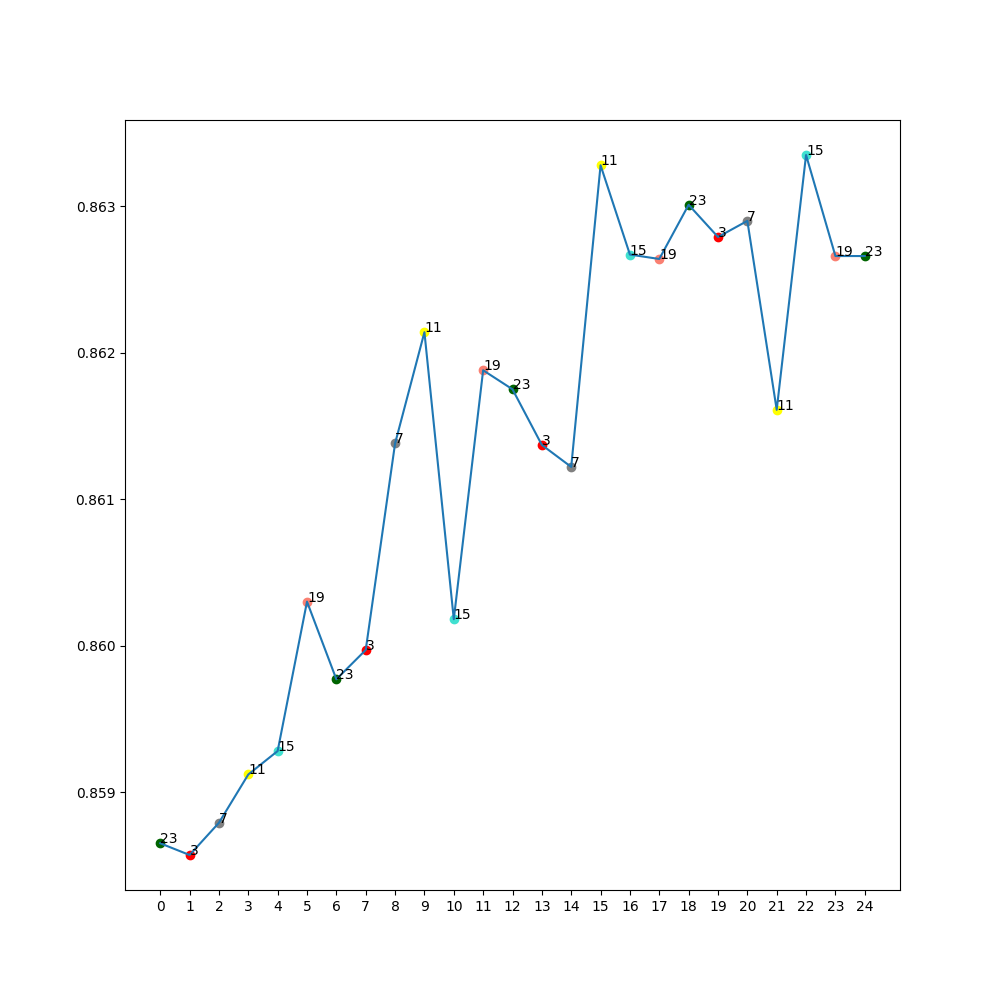
\includegraphics[width=0.8\textwidth]{volumte_time_analysis_linechart.png}
				\caption{Volume Time Analysis}
				\label{fig:volumte_time_analysis_linechart}
			\end{figure}			
			This is a fairly interesting finding as we can see that sometimes the 
			price starts to move very significantly during the busy hour of the London Stock Exchange and we see fairly strong price movements even for one of the most stable markets in the 
			world which is the currency exchange market.
			
			In certain cases like at the 9th and 10th record. The time was 11 and 15 which are the 2 highest trading volumes. We can see that price is moving in a certain direction and then suddenly it changes its direction and starts moving in the opposite direction.
			This is the concept "internal agreement" and it is very interesting to see that the price is moving in a certain direction and then suddenly changes its direction. However it could be 
			explained by the opening of the market and the sheer volume of trading that is happening during these hours is able to change the direction of the market and if the "interna agreement" happened
			the market starts to move uni-directionally.
			In other cases we can
			see that price of the market is stagnating and is not moving at all. This is also a very interesting finding as we can see that the price is not moving at all during the busiest hours of the day, which 
			on the first look could be contradicting the previous finding. However this is not the case as it can easily be exaplained by nullifying the "internal agreement" of the market.
			This case can be seen at the 17th record where we can see that during the busiest trading hour the price is not moving at all.
			The bulls (people that are trying to raise the price up) are not able to overpower the bears (individuals that are selling in order to devalue the trading pair) and the bears are not able to overpower the bulls and therefore the price is not moving at all. 
			

	\section{Machine Learning models}
		\subsection{Neural Network (LSTM)} 
			In this segment I will be focusing on the implementation of the LSTM \cite{lstm_implement} model and trying to determine its performance and analyze its imeplementation.
			LSTM or Long Short Term Memory is a type of Recurrent Neural Network that is able to remember the context of the data and is able to remember the previous data points.
			This feature is very useful for time series forecasting as the model is able to remember the previous data points and is able to predict the future data points based on the previous ones.
			In order to implement the LSTM model I have used the following libraries: Pandas, Numpy, Matplotlib, Plotly, Scikit-learn, Tensorflow

			The main issue when it comes to the implementation of any machine learning model that is trying to predict time-series data is the fact that the traditional golden 80/20 rule does not apply as
			there are local trends which are not applicable to the entire dataset. Therefore I have decided to use a different approach and split the data using a library TimeSeriesSplit from Scikit-learn.
			This way I am going to be able to split the data into multiple splits and train the model on each of the splits. This way I am going to be able to train the model on multiple different trends and
			see different results.
			I have decided to use 6 splits and train the model on each of the splits.
			I have decided to buld the model in the following way:
			\begin{figure}
				\centering
				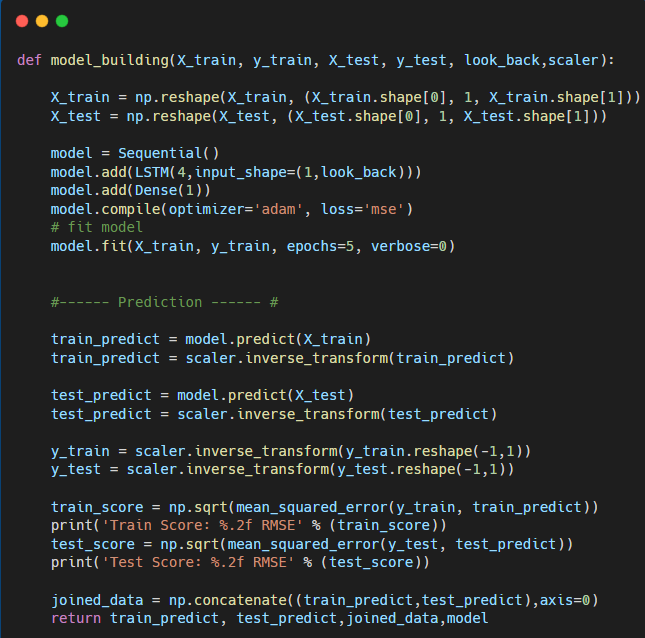
\includegraphics[width=0.8\textwidth]{lstm_code.png}
				\caption{LSTM Model}
				\label{fig:lstm_model}
			\end{figure}
				
		
			I am using a Sequential model which is a linear stack of layers. I am than adding a LSTM
			layer with 4 units and a Dense layer with 1 unit. I am using the Adam optimizer and the Mean Squared Error as a loss function.
			I have decided to use the Adam optimizer as it is a very popular optimizer and is used in many different fields. After fitting the model with the data I am than calling a predict function which is native to the library 
			that I am using. In order to have better results I am than scaling the data using an inverse transform function which does the opposite of the scaling function and scales the data back to its original form. 
			After scaling the data back to its original form I am than calculating the RMSE and R2 score of the model. 
			By running my model on 6 parts of the data I have been able to achieve the following results:			
			\begin{figure}
				\centering
				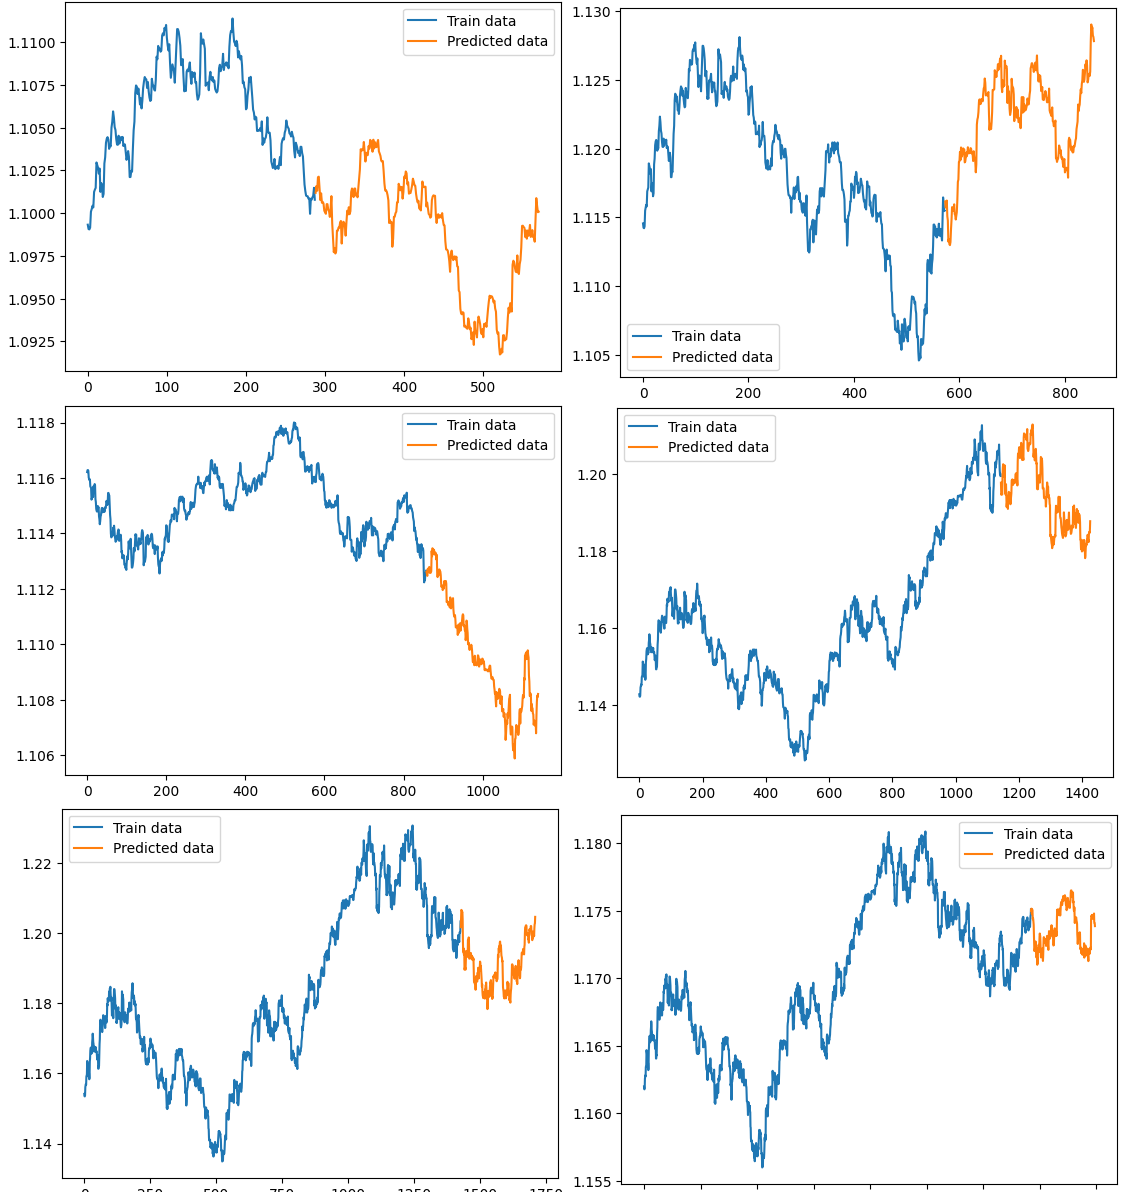
\includegraphics[width=0.8\textwidth]{lstm_chart.png}
				\caption{LSTM Model Results in different splits}
				\label{fig:lstm_model_plots}
			\end{figure}
			As we can see on the plots the plots blue is the actual price of the stock market and the orange is the predicted price of the stock market. The model prediction is very accurate as it is holding the same trend as the actual price
			of the stock market. The test data is the data that the model has not seen before and is used to test the model and see how well it is performing. The model is performing very well on the test data and is able to predict the price of the stock market.
			The average values on the test data are the following: 
			\begin{table}[h!]
					\centering
					\begin{tabular}{|c|c|c|c|c|}
						\hline
						\textbf{MSE} & \textbf{MAE} & \textbf{RMSE}  & \textbf{R2}\\ \hline
						0.0 & 0.012 & 0.014 & 0.029\\ \hline
					
		
					\end{tabular}
					\caption{LSTM Model Results}
					\label{tab:lstm_model_results}
	
			\end{table}


				
			As we can the average MAE is 0.012 is a very good result and is able to predict the price of the stock market with very low error. The R2 score is 0.029 which is also a very good result and is a significant.
			RMSE or Root Mean Squared Erro is the standard deviation of the residuals and in my implementation the results of  0.014 is a very good result and satisfactory.
			with very low error.
		\subsection{ARIMA}
			Autoregressive Integrated Moving Average or industry known as ARIMA is a very popular model used for time series forecasting. It is the most popular model used for time series forecasting and its use cases are very wide due 
			to the fact that during its activation it is combining the usage of 3 different models. ARIMA is a combination of Autoregression, Differencing and Moving Average. The concept of these 3 models was already 
			introduced in the theoretical part of this thesis and therefore I will not be going into detail about them. I will be focusing on the implementation of the ARIMA model and its performance.
			In order to implement the ARIMA model I have used the following libraries: Pandas,statsmodels, Matplotlib, pmdarima and Scikit-learn. Scikit-learn only to calculate MSE and MAE.
			\begin{figure}
				\centering
				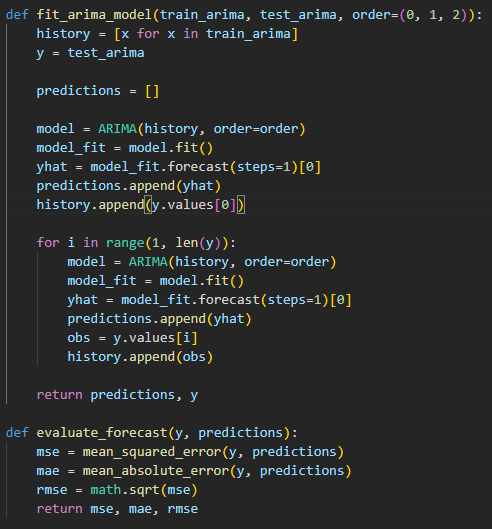
\includegraphics[width=0.8\textwidth]{arima_code.png}
				\caption{ARIMA Model}
				\label{fig:arima_model}		
			\end{figure}
			In order to run the ARIMA model there are 3 main steps that need to be done. The steps is to split the data into train and test data. This is than followed by fitting the model with the train data
			and than predicting the test data.During this step I have been calculating a rolling forecast during which I have builf a new model based on the previous data and than predicted 
			the next data point. This way I was able to predict the entire test data iteratievly and than calculate the RMSE and MAE of the model. There also comes a question of tuning the
			model by optimizing the hyperparameters. In order to do that I have used a library called pmdarima which allowed me to find the best set of hyperparameters for my model.
			The hyperparameters that I have used are the following: 0,1,2. During this function I have also used a native forecast function which is able to predict the future data points.
			By activating of this function I have been able to find yhat which are the predicted values of the future data points. I have than used these values to calculate the RMSE and MAE
			of the model in next step.
			
			\begin{figure}
				\centering
				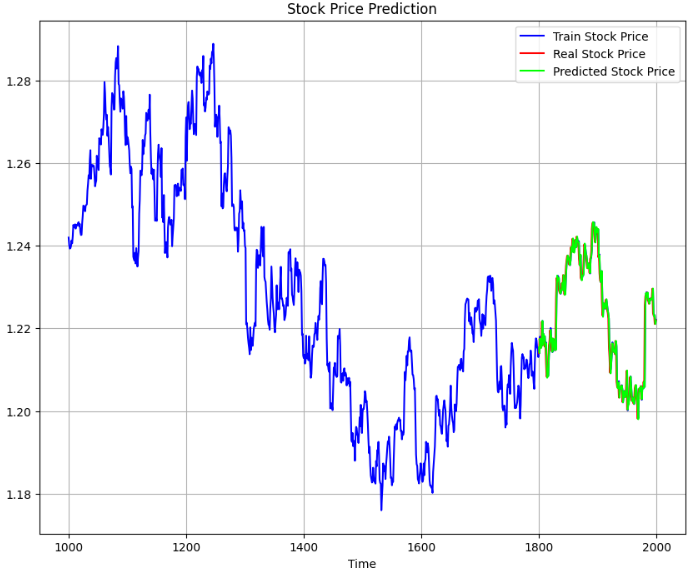
\includegraphics[width=0.8\textwidth]{arima_chart.png}
				\caption{ARIMA Model Results}
				\label{fig:arima_model_plots}
			\end{figure}

			On this chart we can see 3 colors blue green and red being train data, predicted data and test data respectively. On this plot we can see that the predicted data is very much following  
			the real data at the end. This is a very good sign as it means that the model is able to predict the future data points with low error. The model is performing very well on the test data. 
			I have personally had a expectation that the model will be performing very well as it is very widely used and is known in the Machine Learning community as the best model for time series forecasting.
			My exectations were not hindered and the model was able to achieve the following metrics for MSE,MAE and RMSE.
			\begin{table}[h!]
				\centering
				\begin{tabular}{|c|c|c|c|c|}
					\hline
					\textbf{MSE} & \textbf{MAE} & \textbf{RMSE}  & \textbf{R2}\\ \hline
					8.489e-06 & 0.002 & 0.003 & 0.952\\ \hline
				\end{tabular}
				\caption{ARIMA Model Results}
				\label{tab:arima_model_results}
			\end{table}

			Judging by the results the model is performing very well and is able to predict the future data points with very low errorr and is able to predict the future price of the stock market.
			
	
		
		\subsection{XGBoost}
			XGBoost or also known as Extreme Gradient Boosting is machine learning model that is used for both classification and regression problems. XGBoost as an algorithm uses an ensemble of decision trees
			and implements a gradient boosting framework. The gradient boosting framework is an approach where new models are created that predict the residuals or errors of prior models and then added together.
			This means that over time the model is taking the errors of the previous models as inputs and is trying to predict the errors of th next model. This way the model is able to learn from its mistakes and improve every
			iteration. In order to implement the XGBoost model \cite{xgboost_implement} I have used the following libraries: Pandas, Numpy, Matplotlib, Plotly, Scikit-learn and XGBoost. 
			\begin{figure}[h]
				\centering
				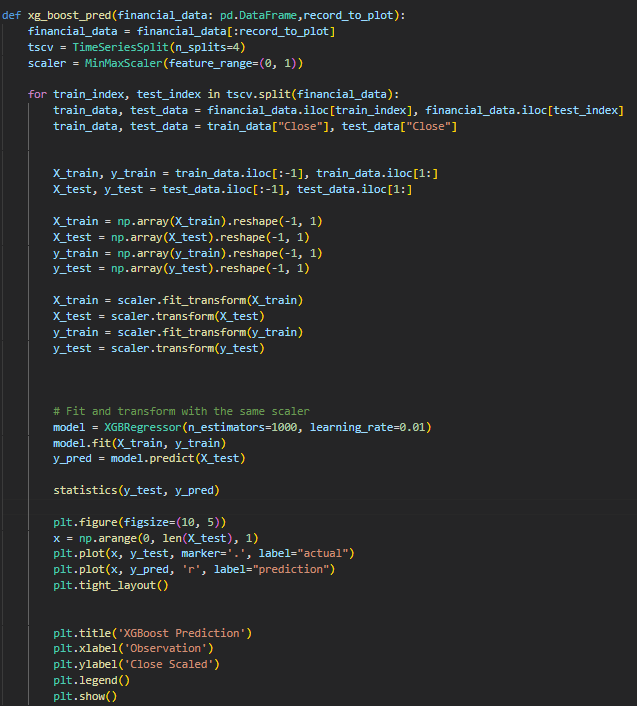
\includegraphics[width=0.8\textwidth]{xgboost_code.png}
				\caption{XGBoost Model}
				\label{fig:xgboost_model}
			\end{figure}

			In my implementation I have also decided to use the time series split as I have done previously. The train test split is the same as in the previous models. What changed is that now I have decided to use 
			scaler transform and fit transform for my train and test data respectively. This will allow me to scale the data and make it more suitable for the model. I have also decided to use a MinMaxScaler which takes 
			the data and scales it to a range of 0 and 1. By scaling the data I am able to make the data more suitable for the model and therefore improve its performance. When it comes to building the model I have decided not to define
			anything as an initial value. In order to experimentater. Internally the objective of this model is squared error and therefore there is not neeed to overwrite it. After building the model, I have decided to 
			experiment with hyperparameters, specifically: number of estimators, learning rate, max depth, subsample and colsample bytree. Running this hyperparameter tuning was very time consuming and took a lot of time to run. 
			\begin{figure}[h]
				\centering
				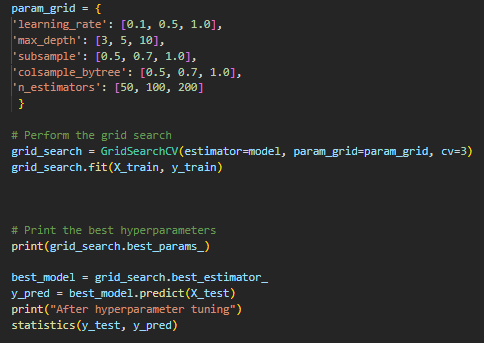
\includegraphics[width=0.8\textwidth]{xgboost_tuning_code.png}
				\caption{XGBoost Hyperparameters}
				\label{fig:xgboost_hyperparameters}
			\end{figure}
			As we can see from the code I have decided to use a GridSearchCV which is a function that is able to run a grid search on the hyperparameters and find the best set of hyperparameters for my model.
			The input parameter of cv is representing a cross-validation which is a technique used to evaluate the performance of the model. I have decided to use a 3 fold cross validation which means that the data is split into 3 parts and
			the model is trained on 2 parts and tested on 1 part. This is done 3 times and the average of the 3 results is taken. This way I am able to evaluate the performance of the model on multiple different splits and therefore.
			By doing this and also time-series split I am evaluate the perfromance exceptionally well as I am doing it natively by taking 4 parts in the outer loop and than each of those 4 parts has the cross-validation actiavted on top of it.
			The concept of trying to find the hyperparameters is great however when trying to hard we can overfit the model and therefore the model will not be able to generalize well. This is why I have decided to use a 3 fold cross validation.
			By trying too hard we are encountering a well known issue in the machine learning world wchich is called: Bias Variance Tradeoff. This is a very important concept in the machine learning world and is used to describe the problem of overfitting
			and underfitting. 
			\begin{figure}[h]
				\centering
				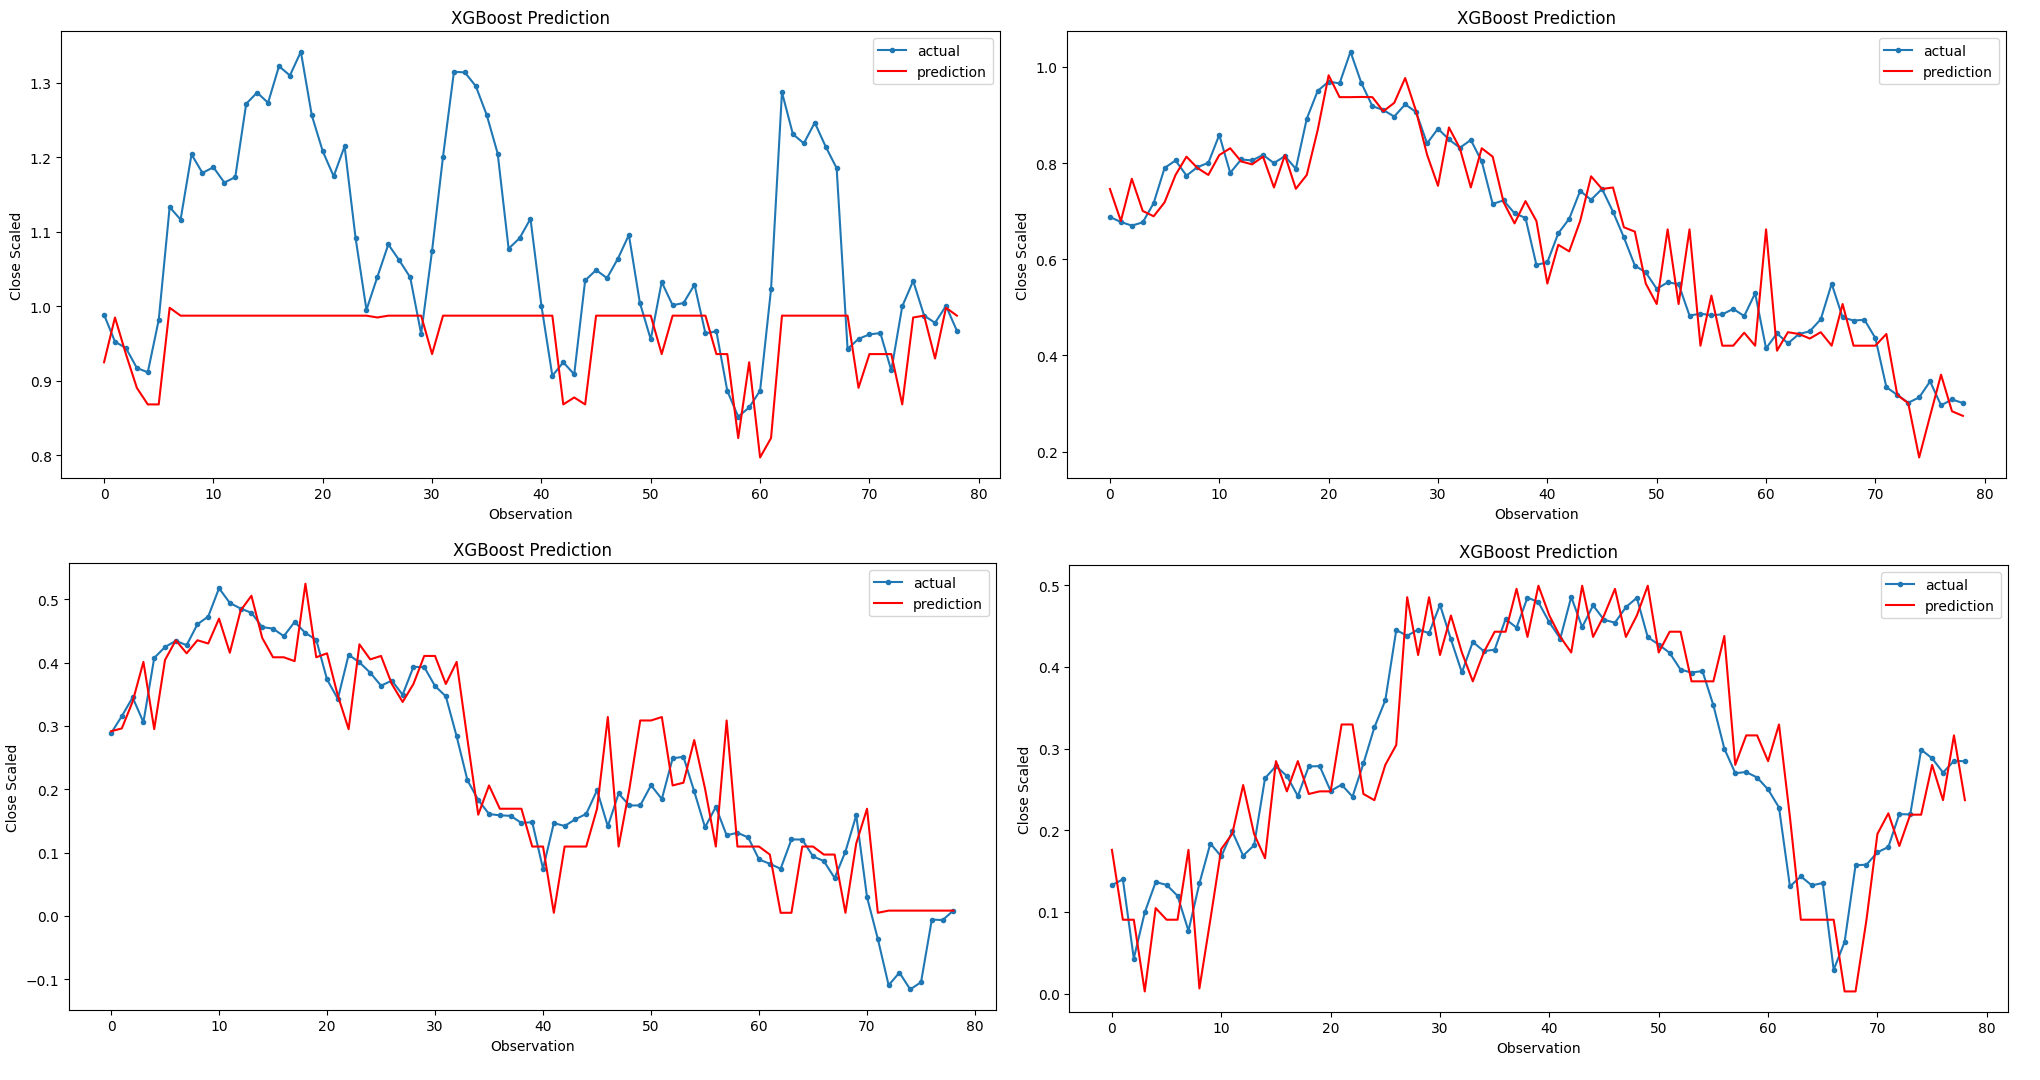
\includegraphics[width=0.8\textwidth]{xgboost_chart.png}
				\caption{XGBoost Chart}
				\label{fig:xgboost_chart}
			\end{figure}
			On this plot we can see perfroamce on XGBoost model over the 4 splits we initialized at the start. The blue line is the actual price of the stock market and the orange line is the predicted price of the stock market.
			We can see that on the first figure the model is basically skipping over the extreme values and plateauing. This is a very interesting finding as it means that the model is not able to predict the extreme values and is not able to predict the 
			movement in some cases. On the other hand the other 3 figures are being tracked exceptionally well, even though we can see a small offset in the 3rd figure. This is a very good sign as it means that the model is able to have an 
			advanced grasp of what is going on in the market. The performance of this model was collected in this table. All the values in the table are the average of the 4 splits.
			\begin{table}[h]
				\centering
				\begin{tabular}{|c|c|c|c|}
					\hline
					\textbf{MAE} & \textbf{MSE} & \textbf{RMSE} & \textbf{R2} \\ \hline
					0.068 & 0.098 & 0.089 & 0.50 \\ \hline
				\end{tabular}
				\caption{XGBoost Detailed Results}
				\label{tab:xgboost_detailed_results}
			\end{table}
			From the detailed information that were collected we can see that MAE(Mean Average Eror), MSE(Mean Squared Error) and RMSE(Root Mean Squared Error) are very low which is a very good sign. The only concerning metric is the R2 score which is 0.5.
			This is not particularly bad however it is not particularly good either. The R2 score is a metric that is used to measure the variance of the data and therefore it could also just indicate the market has high variance and that is the 
			sole reason why the R2 is higher. Conclusion to XGBoost: XGBoost has a great performance and our expectation were met as it a solid machine learning model with a rational logic backing it.
		\subsection{Support Vector Regression}
			Support Vector Regression or industry known as SVR \cite{svr_implement} is machine learning model that is used for regression problems. It belongs to the family of Support Vector Machines and is working on the 
			principle of trying to find the best fit line that is able to fit the data. SVR is used for continuous data and is able to predict the future data points. It could be Mathematicaly represented as:
			\begin{equation}
				y = \sum_{i=1}^{n} \alpha_i K(x_i,x) + b
			\end{equation}
			Where:
			\begin{itemize}
				\item $y$ is the predicted value
				\item  $\alpha$ is the weight 
				\item  $K$ is the kernel function
				\item  $x_i$ is the training data
				\item  $x$ is the test data.

			\end{itemize}
			SVR is offering a series of different kernels that can be used to fit the data. The most popular ones are: Linear, Polynomial, RBF and Sigmoid.
			In my implementation I have decided to use the RBF, Linear and Polynomial kernel and compare their performance. In order to implement the SVR model I have decided to use the time series split as I have done with the LSTM model.
			I have decided to use only 4 splits and look at a very short time period of 100 ticks. I have decided to use a short time period as I wanted to see how the model is performing on a short time period and how it is able to perform 
			on a short training data. The implementation of the SVR is rather simple and it can be done like this:
			\begin{figure}[h]
				\centering
				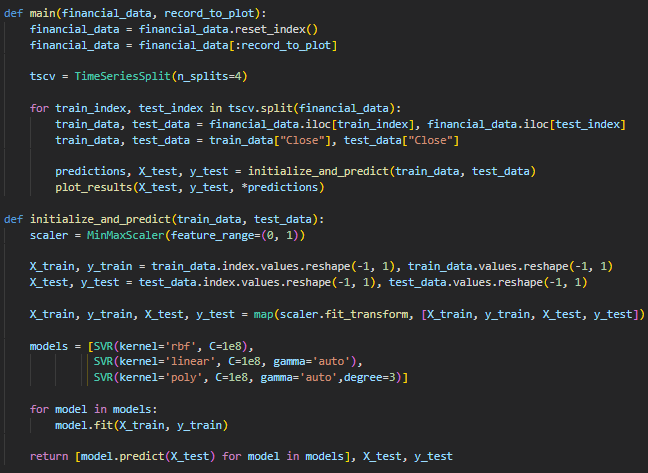
\includegraphics[width=0.8\textwidth]{svr_code.png}
				\caption{SVR Model}
				\label{fig:svr_model}
			\end{figure}
			At the start I have declared 4 time series splits and looped through each of them. I have than declared 3 different models (RBF, Linear, Polynomial) and than fitted each of them with the train data.
			In terms of the hyperparameters I have opted to minimize the C as I am dealing with very litle changes in the data over time. The principle of C is that it is a penalty parameter of the error term.
			It controls the trade off between smooth decision boundary and classifying the training points correctly. As my deltas are very small I have decided to minimize the C and therefore minimize the penalty parameter. 
			In terms of the gamma I have decided to use go for the auto option for the Linear and Polynomial kernels and for RBF I have decided to use the scale option. I have also decided to use a scaling function
			provided by a library Scikit-learn. In my implementation I have decided to use a MinMaxScaler which takes the data and scales it to a range of 0 and 1. This is a very useful function as it is able to scale the data 
			irrelevant of its magnitude. As my percentage changes are very small this scaler is going to be very useful for my implementation.
			The largest drawback I have found with the SVR model is the fact that it is very slow and it takes a lot of time to train the model when using extremely low values of C. 
			After fitting the model I have than predicted the test data and calculated the RMSE and MAE of the model.
			\begin{figure}[h]
				\centering
				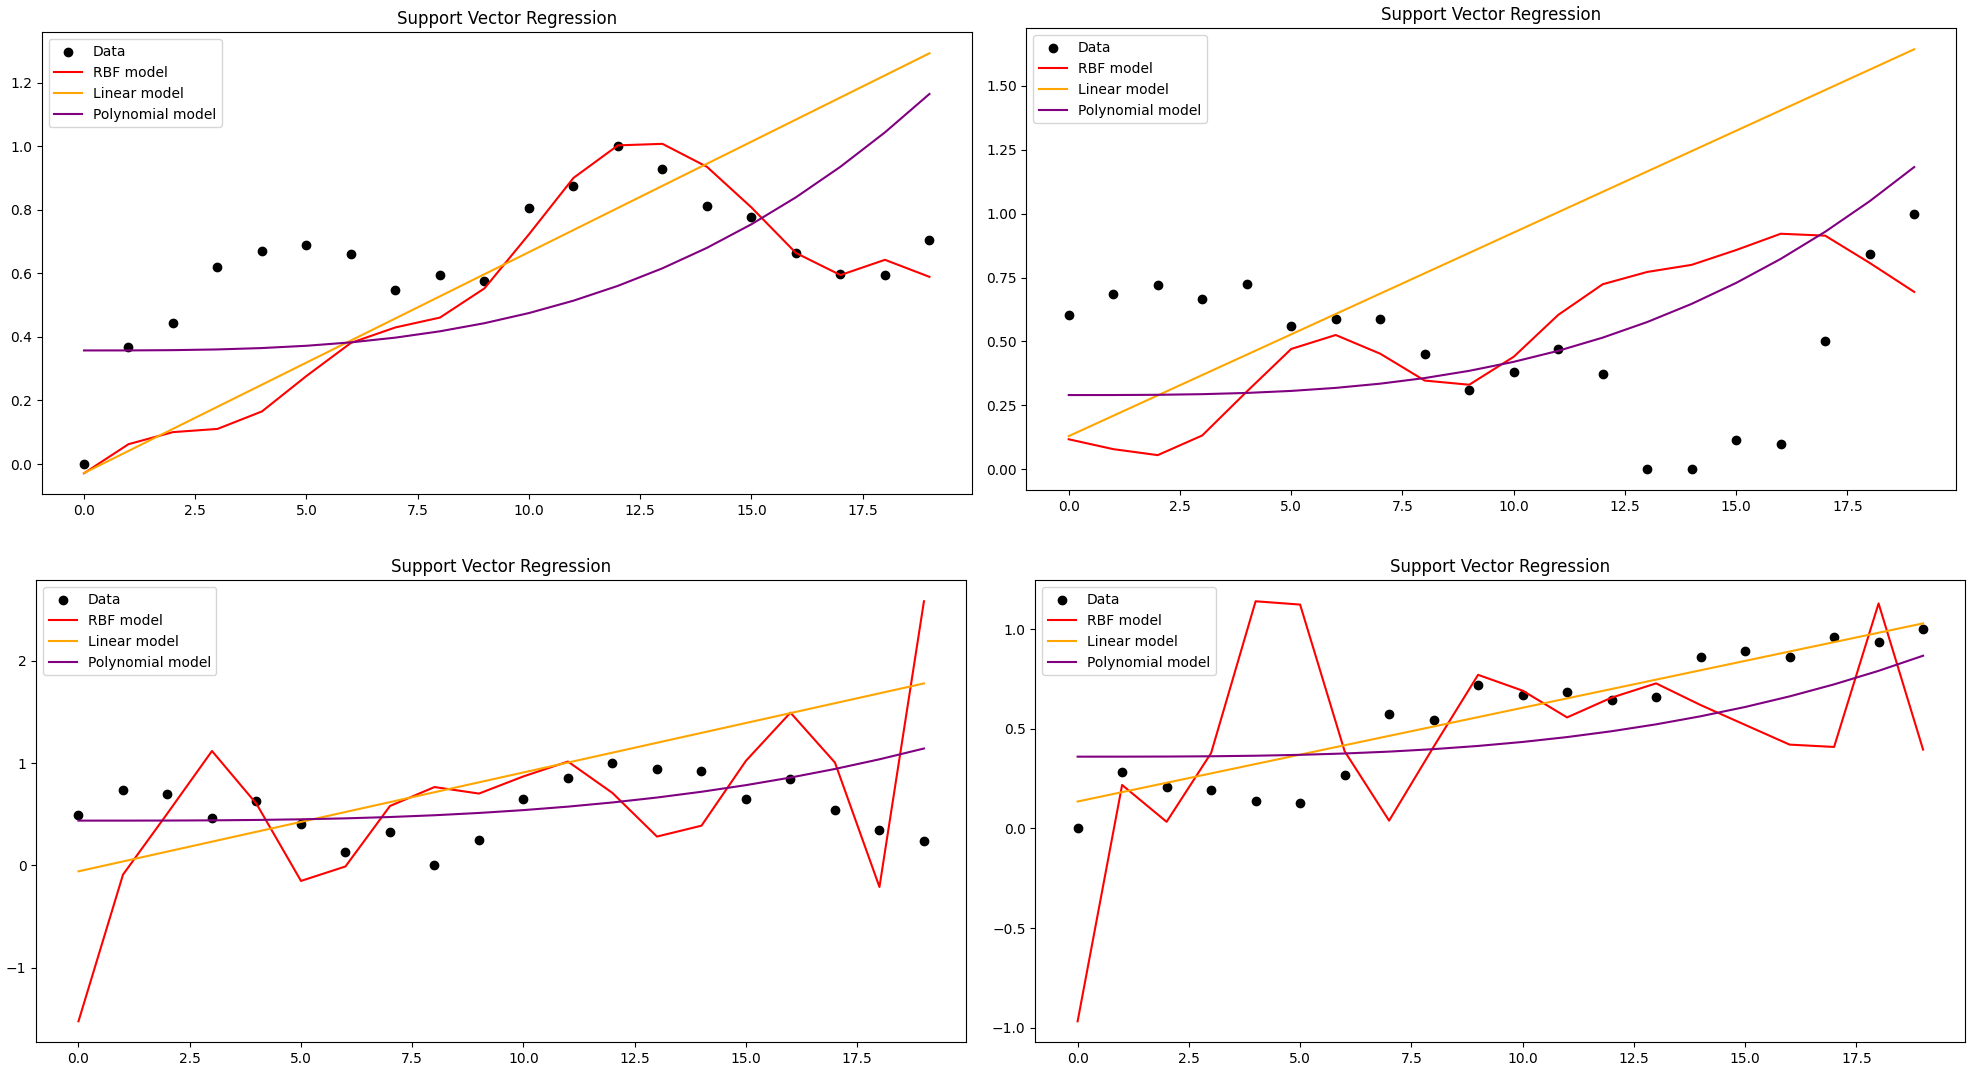
\includegraphics[width=0.8\textwidth]{svr_chart.png}
				\caption{SVR Model Results}
				\label{fig:svr_model_plots}
			\end{figure}
			On this plot we can see the actual price of the stock market as a black scatter plot and 3 lines which are trying to preedict the movement of the stock market. Red is the RBF kernel, orange is the Linear kernel and purple is the Polynomial kernel.
			As we can see the RBF kernel is on the first look performing the best and is able to predict the market with the closest match to the actual price. The Linear kernel is performing the worst and is not able to predict the market at all.
			The performance of the Polynomial kernel is questionable however it is relatively successful in predicting the market. Each of the 4 plots is representing a different split and therefore we can see that the model is performing differently on each of the splits.
			Its performance can be summarized in the following table where we can see MSE, MAE and R2 score of each of the kernels. The data inside of this table is the average of the 4 splits.
			
			
			\begin{table}[h!]
				\centering
				\begin{tabular}{|c|c|c|c|c|}
					\hline
					\textbf{Type} & \textbf{MSE} & \textbf{MAE} & \textbf{R2} & \textbf{RMSE} \\ \hline
					RBF & 0.297 & 0.371 & -2.866 & 0.500 \\ \hline
					Linear & 0.268 & 0.374 & -2.854 & 0.454\\ \hline
					Poly & 0.099 & 0.099 & -0.483 &  0.308 \\ \hline
				\end{tabular}
				\caption{SVR Model Results}
				\label{tab:svr_model_results}
			\end{table}
			After carefully examining the averages and comparing the results with the plots we can see that statistically the Polynomial kernel is performing the best. However the RBF kernel is performing the best on the plots.
			 The perfromance of the Linear kernel is almost identical to the RBF kernel however when lookin at the plots we can clearly see that the RBF kernel is performing better. The reason for this could be the fact that the RBF kernel has higher variance
			 when it start to predict the future data points and the initial prediction is not very close to the actual price. However as the prediction continues the RBF kernel is able to predict the future data points with higher accuracy, 
			 but tends to fly off the actual price at the end. As a conclusion we can say that the SVR model is not performing very well and could not be used for time series forecasting. The reason for this could be the fact that the SVR model is not able to 
			accurately detect trends and match the data flow of the stock market.

	\section{Technical indicators}
		\subsection{RSI}
			RSI stands for Relative Strength Index and is a momentum indicator used in technical analysis that measures the magnitude of recent price changes to
			evaluate overbought or oversold conditions in the price of a stock or other asset. RSI is one of the most popular technical indicators
			and works on the principle of moment where we define a delta, gain and loss. The formula for calculating the RSI is the following:
			\begin{equation}
				RSI = 100 - \frac{100}{1 + RS}
			\end{equation}
			Where:
			\begin{itemize}
				\item $RS = \frac{Average\ Gain}{Average\ Loss}$
				\item $Average\ Gain = \frac{Sum\ of\ Gains\ over\ the\ past\ X\ periods}{X}$
				\item $Average\ Loss = \frac{Sum\ of\ Losses\ over\ the\ past\ X\ periods}{X}$
			\end{itemize}

			
			It can be clearly seen that RSI \cite{rsi_implement}is working on the principle of momentum due to the fact it is using the previous X periods and is calculating the average gain and loss.
			By using the average gain and loss we are able to calculate the RS and then the RSI. The RSI is an actual number between 0 and 100 and is used to determine if the market is overbought or oversold.
			When the RSI is above a ceratin factor we do consider the market to be overbought and when the RSI is below a certain factor we do consider the market to be oversold.
			In my implementation iam using a factor of 4. I am than using factor in my implementation to adjust the RSI values at crossover and crossunder points to make the indicator
			more responsive to changes in the market.
			\begin {figure}[h!]
				\centering
				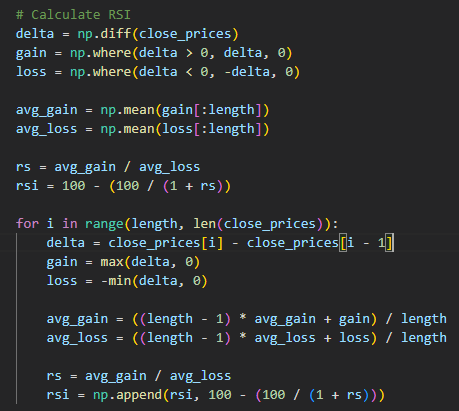
\includegraphics[width=0.8\textwidth]{rsi_code.png}
				\caption{RSI}
				\label{fig:rsi}
			\end {figure}
			My implementation is not only limited to the usage of RSI, but I am also incorporating the usage of Trailing Stop.
			At the begining of the implementation I am setting the initial values of crossover and crossunder where for each index RSI is lower or higher than 1.
			\begin{figure}[h!]
				\centering
				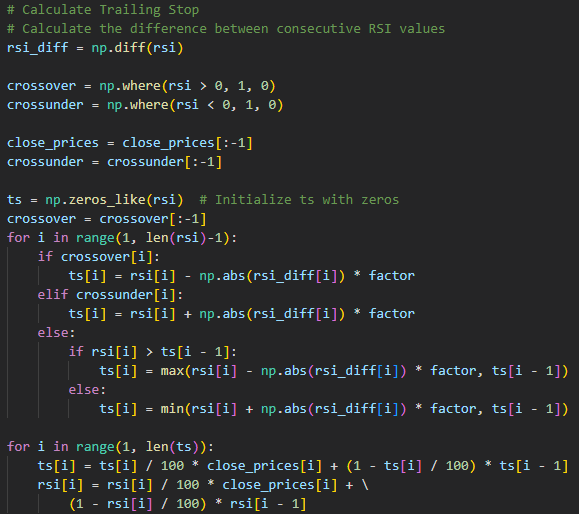
\includegraphics[width=0.8\textwidth]{trailing_stop.png}
				\caption{RSI}
				\label{fig:rsi_initial_values}
			\end{figure}
			If the crossover or crossunder is detected by the presence of a 1 at the current index a Trailing Stop is calulated. It is calculated by
			the difference between the RSI value at the current index and the absolute value of the RSI at the current index multiplied by the factor mentioned before.
			After successfully calculating the Trailing Stop we are than reassinging the values of RSI and Trailing Stop in the following way. Combining a 
			percentage of the current value with a percentage of the previous value, weighted by the corresponding close price.
			After calculating the trailing stop I have than decided to apply smoothening to the RSI values in order to make the indicator once again
			more responsive to changes in the market and not be as volatile.
			Throughout my entire research section with the Technical Indicators I am going to be also detecting the signals of buy and sell.
			These signals are important for the Backtesting module and its input as it relies on concrete signal to determine whether to buy or sell.
			In my RSI strategy the buy signal is executed when the smoothed RSI is higher than the trailing stop and the sell signal is executed when the
			smoothed RSI is lower than the trailing stop. 
			\subsubsection{Performance}
				
				In terms of performance. RSI had a great performance on the provided data and was able to detect trend changes very well. On the plot we can
				see the buy signals as green dots and the sell signals as red dots.
				\begin{figure}[h!]
					\centering
					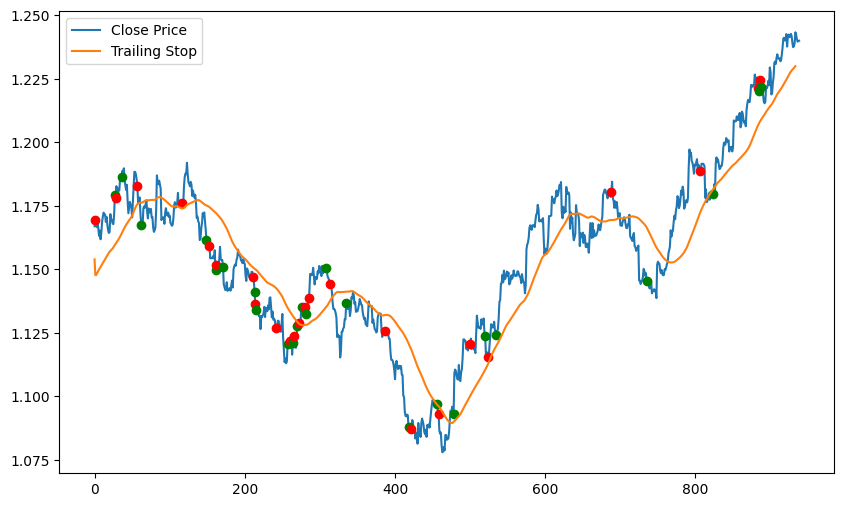
\includegraphics[width=0.8\textwidth]{rsi_plot.png}
					\caption{RSI Performance}
					\label{fig:rsi_performance}	
				\end{figure}

				The buy signals are executed when the RSI is higher than the trailing stop
				and the sell signals are executed when the RSI is lower than the trailing stop. 
				Over the span of 4000 hours, the RSI was able to achieve the following metrics
				\begin{table}[h!]
					\centering
					\begin{tabular}{|c|c|c|c|c|}
						\hline
						\textbf{ROI} & \textbf{Win Rate} & \textbf{Buy \& Hold Return} & \textbf{Average Trade Return} \\ \hline
						17.4\%         & 95.7\%               & 10.6\%                         & 2.5\%                           \\ \hline
					\end{tabular}
					\caption{RSI Performance Metrics}
					\label{tab:rsi_performance_metrics}
				\end{table}

				Overall performance of RSI could be rated as very successful as it was able to generate a return on investment of 17.4\% and a win rate of 95.7\%.
				Even though the market has grown by 10.6\% during the same time period. The RSI was able to outperform the market by almost 7\% which is a very
				significant difference on a low volatile market like the currency exchange one.
		

		\subsection{Bollinger Bands}
			Bollinger Bands are a well known technical indicator that is used to determine the volatility of the market. It was created by John Bollinger in the 1980s.
			Bollinger Bands is a technical analysis tools comprising of two regions that are signalizing the volatility of the market. The first region is the upper band
			which is signalizing the overbought region and the second region is the lower band which is signalizing the oversold region. The middle band is signalizing the
			moving average of the market. As described Bollinger bands are composed of 3 lines. The upper band, the lower band and the middle band. 
			\begin{itemize}

				\item The middle band can be represented as the following:
					\begin{equation}
						Middle\ Band = \frac{Sum\ of\ Close\ Prices}{Number\ of\ Periods}
					\end{equation}
					Where the number of periods is the number of periods we are using to calculate the moving average. In my implementation I am using 50 periods. 
					The number 50 was picked as I am trying to work on larger scale rather than short term swings that introduce extreme volatility due to the increased trading volume
					by hedge funds and other large financial institutions. 

				\item The upper band can be represented as the following:
					\begin{equation}
						Upper\ Band = Middle\ Band + 2 * Standard\ Deviation
					\end{equation}
					Where the middle band is the moving average of the market and the standard deviation is the standard deviation of the market at the current index.
				\item The lower band can be represented as the following:
					\begin{equation}
						Lower\ Band = Middle\ Band - 2 * Standard\ Deviation
					\end{equation}
			\end{itemize}
			
			\begin{figure}[h!]
				\centering
				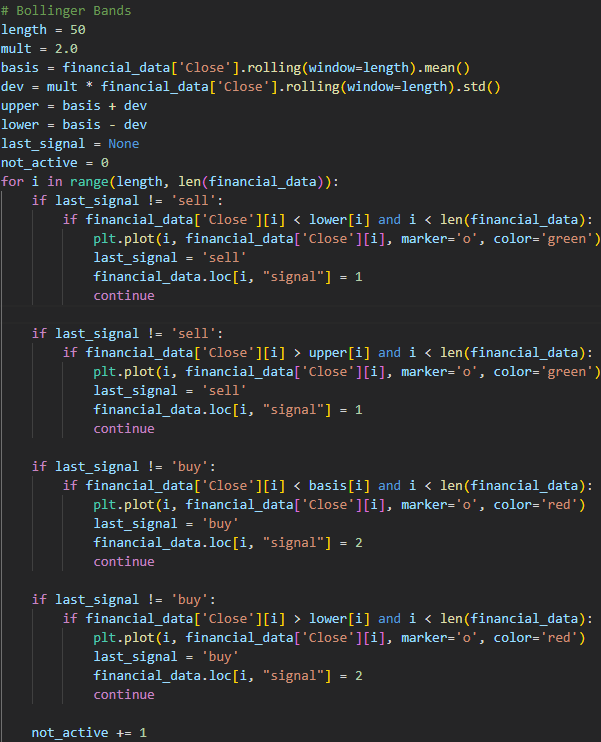
\includegraphics[width=0.8\textwidth]{bollinger_bands_code.png}
				\caption{Bollinger Bands}
				\label{fig:bollinger_bands}

			\end{figure}
			As we can see from the formulas above the Bollinger Bands are working on the principle of volatility.
			At the begining of the implementation I am setting the length and the number of standard deviations. The length is the number of periods we are using to calculate
			the moving average. The variable basis is than used to calculate the rolling mean of the window we have specified and the variable dev 
			has the same purpose but is used to calculate the rolling window of the standard deviation.
			After successfully calculating the rolling mean and the rolling standard deviation we are than calculating the upper and lower band. By
			summing or subtracting the rolling mean with the rolling standard deviation respectively.
			
			\subsubsection{Trend detection}
				The trend reversal into an uptrend is signaled when the Close price is below the lower band and the previous signal was a buying signal
				The trend reversal into a downtrend is signaled when the Close price is above the upper band and the previous signal was a selling signal
				
				I have opted to have 2 buy and sell detection cases
				\begin{itemize}
					\item The first buy: The first buy happens when the close price is below the basis and the previous signal was a sell.
						\subitem This case is used to detect when the price could be called a safe buy and is used to detect when the price is in the oversold.
						region and we are entering based on the moving average.
					\item The second buy: The second buy happens when the close price is higher than the lower band and the previous signal was a sell. 
						\subitem This case is used to detect sharp trend reversals and is used to detect when price starts to recover after being tanked by the bears. 
					\item The first sell: The first sell happens when the close price is higher than the upper band and the previous signal was a buy.
						\subitem This case is used to detect when the price could be called a must sell and is used to detect when the price have shot up massively and 
						is even outside of the overbought region.
					\item The second sell: The second sell happens when the close price is lower than the lower band and the previous signal was a buy.
						\subitem This case is used to detect sharp trend reversals and we are trying to protect our profits and sell before the price starts to tank.
				\end{itemize}

			\subsubsection{Performance}
				\begin{figure}[h!]
					\centering
					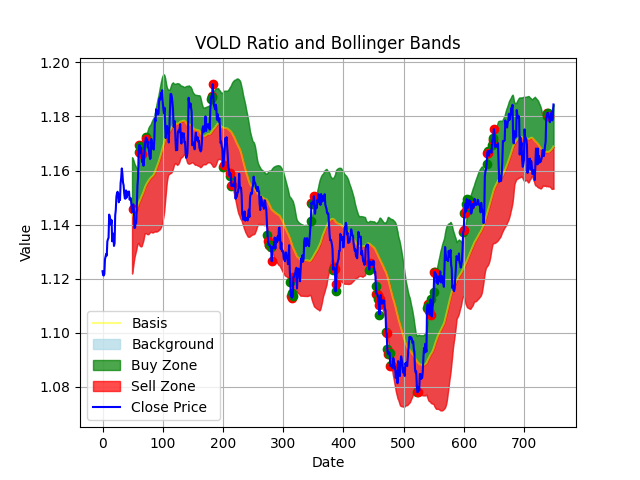
\includegraphics[width=0.8\textwidth]{bollinger_bands_plot.png}
					\caption{Bollinger Bands Performance}
					\label{fig:bollinger_bands_performance}
				\end{figure}
				Bollinger Bands had a very good performance on the provided data and was able to detect trend changes exceptionally well. 
				On the plot we can see a 2 clearly distinct regions (green and red). The green region is signalizing the overbought region and the red
				region is signalizing the oversold region.
				They are split in the middle by a yellow line which is the moving average of the market. 
				
				The metrics of the Bollinger Bands are the following:
				\begin{table}[h!]
					\centering
					\begin{tabular}{|c|c|c|c|c|}
						\hline
						\textbf{ROI} & \textbf{Win Rate} & \textbf{Buy \& Hold Return} & \textbf{Average Trade Return} \\ \hline
						20.5\%         & 92.6\%               & 5.5\%                         & 2.4\%                           \\ \hline
					\end{tabular}
					\caption{Bollinger Bands Performance Metrics}
					\label{tab:bollinger_bands_performance_metrics}
				
				\end{table}
				Overall performance of Bollinger Bands could be rated as very successful as it was able to generate a return on investment of 20.5\% and a win rate of 92.6\%.
				Even when the market has grown by 5.5\% during the same time period. The Bollinger Bands was able to outperform the market by 15\% which could be considered as
				an astonishing result.
		\subsection{Rolling Windows}
			Rolling Windows is a technical indicator which works on a different principle than any other indicator as it work on the principle of peaks and walleys of the market.
			The principle of this indicator is to calculate the where the peaks and walleys of the market are and than calculate the differences between the peaks and walleys.
			When calculating each of the peaks and walleys we are than setting a using the window size in which we are going to be trying to detect the peaks and walleys.
			When trying to detect the peaks and walleys we are using a peak/valley coefficient in order to determine how big of a peak we are trying to detect and how big of a valley we are trying to detect.
			\begin{figure}[h!]
				\centering
				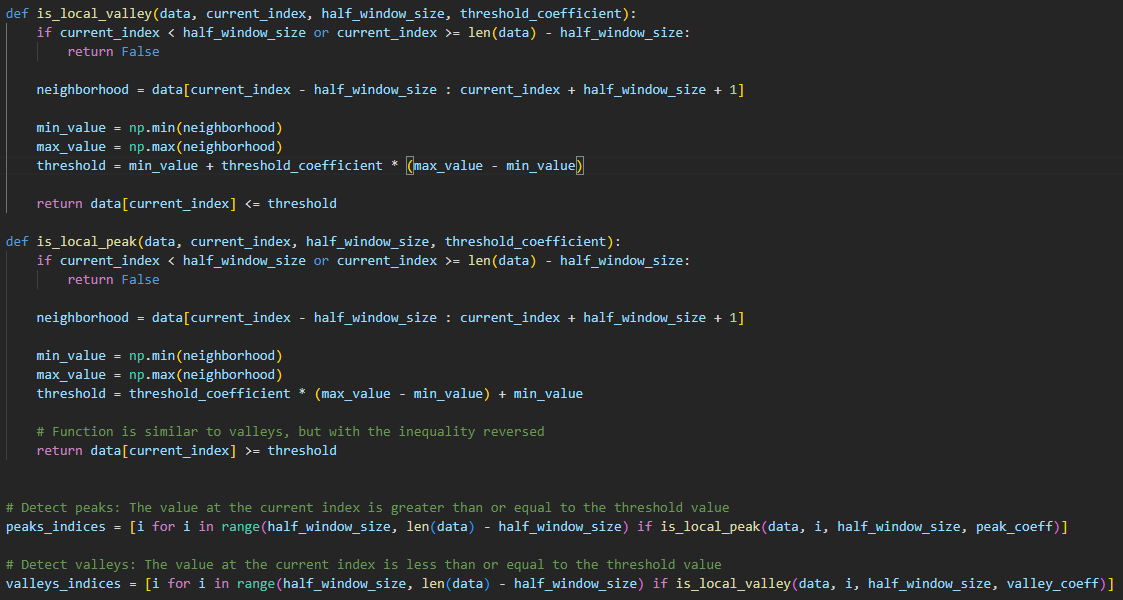
\includegraphics[width=0.8\textwidth]{rolling_windows_code.png}
				\caption{Rolling Windows}
				\label{fig:rolling_windows}

			\end{figure}
			In my implementation you can see 2 clear function which are then used inside of a list comprehension. The first function is local valley in which 
			we are determining a so called neighborhood of the current index by using a half window size in order to determing the neighborhood before and after the current index.
			After successfully determining the neighborhood I am than checking for the lowest and highest value and than determining a threshold. This threshold is than used to determine
			where the value at a current index is confirmed to be a valley or not. If the value at the current index is lower than the threshold it is confirmed to be a valley.
			The second function is local peak which works on the same principle however the only difference is that we are checking if the value at the current index is higher than the threshold.
			The 2 list comprehensions at the end are used to determine the peaks and valleys inside of the entire data frame.
			The three variables that are used to determine the peaks and valleys are the following:
			Peak coefficient: The magnitude of the peak we are trying to detect
			Valley coefficient: The magnitude of the valley we are trying to detect
			Window size: The size of the window we are using to detect the peaks and valleys
			
			Threshold is calculated in the following way:
			\begin{equation}
				Threshold = Threshold\ coefficient * (max\_value - min\_value) + min\_value 
			\end{equation}
			Where:
			\begin{itemize}
				\item $Threshold\ coefficient$ is the coefficient used to determine the threshold
				\item $max\_value$ is the maximum value in the neighborhood
				\item $min\_value$ is the minimum value in the neighborhood
			\end{itemize}
			Peak detection could be represented as the following:
			\begin{equation}
				Peak = \left\{Close\ Price_{i}\right\}_{i=1}^{n} > Threshold
			\end{equation}
			Where:
			\begin{itemize}
				\item $Close\ Price_{i}$ is the close price at the current index
				\item $Threshold$ is the threshold calculated in the previous equation
			\end{itemize}
			Valley detection could be represented as the following:
			\begin{equation}
				Valley = \left\{Close\ Price_{i}\right\}_{i=1}^{n} < Threshold
			\end{equation}
			Where:
			\begin{itemize}
				\item $Close\ Price_{i}$ is the close price at the current index
				\item $Threshold$ is the threshold calculated in the previous equation
			\end{itemize}
			\subsubsection{Trend detection}
				Buy signal is executed when the current value is a confirmed valley and the previous value was a peak.
				Sell signal is executed when the current value is a confirmed peak and the previous value was a valley.
		
			\subsubsection{Performance}
				The performance of this indicator was fairly good and also very interesting idea behind it. The idea of using peaks and walleys to determine the trend of the market
				is a sophisticated idea and its usage could be used with other indicators in pair. Its performance alone was sufficient however I believe that it would be 
				better used alongside other indicators.
				\begin{figure}[h!]
					\centering
					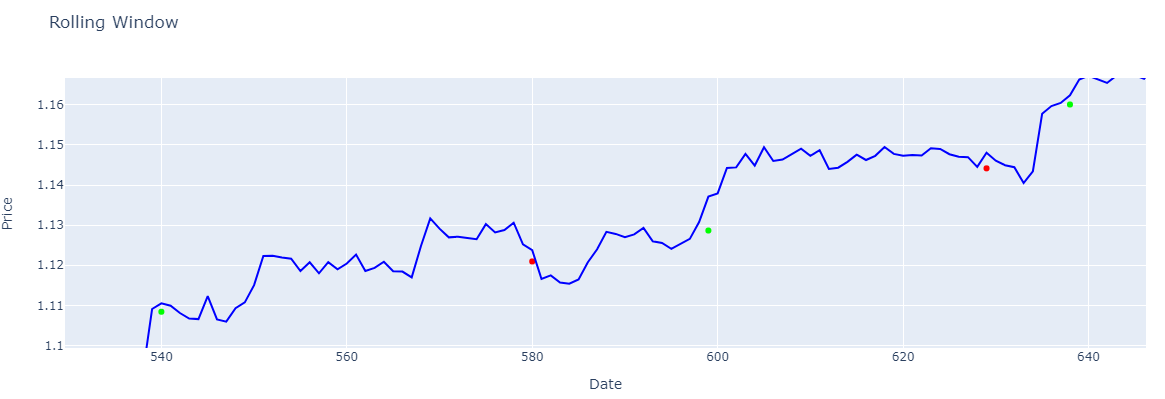
\includegraphics[width=0.8\textwidth]{rolling_windows_plot.png}
					\caption{Rolling Windows Performance}
					\label{fig:rolling_windows_performance}
				\end{figure}
				
				The metrics of the Rolling Windows are the following:	


				\begin{table}[h!]
					\centering
					\begin{tabular}{|c|c|c|c|c|}
						\hline
						\textbf{ROI} & \textbf{Win Rate} & \textbf{Buy \& Hold Return} & \textbf{Average Trade Return} \\ \hline
						20.0\%         & 90.5\%               & 10.6\%                         & 2.8\%                           \\ \hline
					\end{tabular}
					\caption{Rolling Windows Performance Metrics}
					\label{tab:rolling_windows_performance_metrics}
				\end{table}
				The most impressive feature of this algorithm is the constant growth and not a lot of draw backs in terms of final equity.
				On this chart we can see an equity curve of the Rolling Windows algorithm. The equity curve is a graphical representation of the change in value of a trading account over an entire
				time the algorithm was running.
				\begin{figure}[h!]
					\centering
					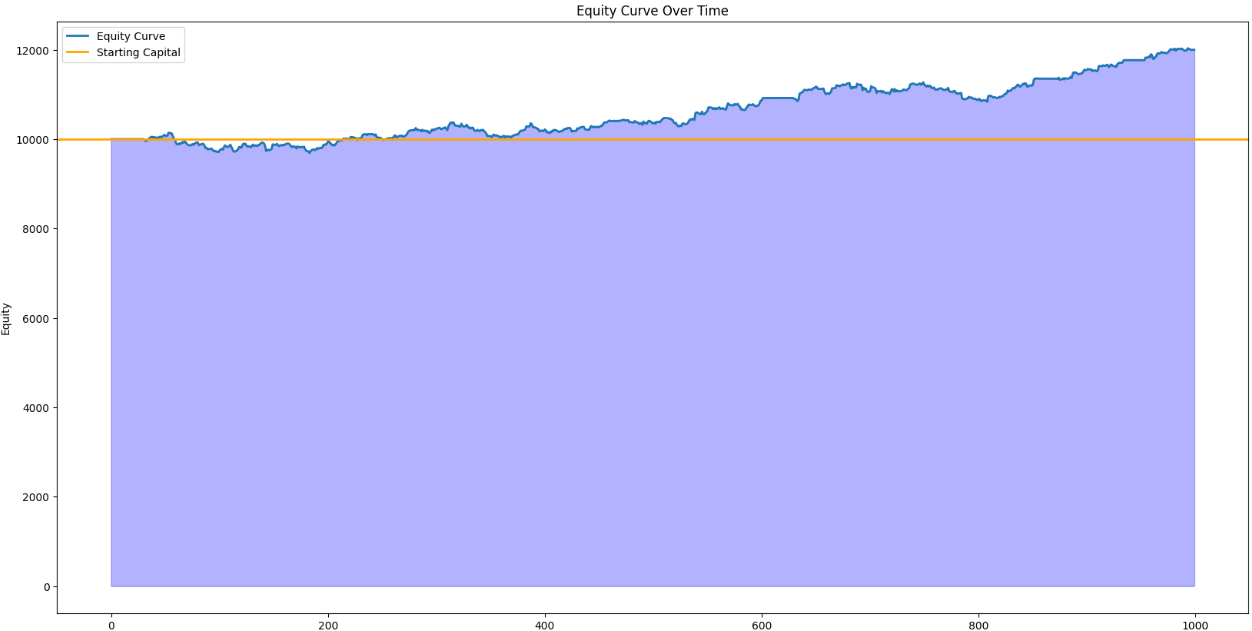
\includegraphics[width=0.8\textwidth]{rolling_windows_equity_curve.png}
					\caption{Rolling Windows Equity Curve}
					\label{fig:rolling_windows_equity_curve}
				Oveall performance of Rolling Windows could be rated as very successful as it was able to generate a return on investment of 20.0\% and a win rate of 90.5\%. 
				Even when the market has grown by 10.6\% during the same time period. The Rolling Windows was able to outperform the market by 9.4\% which could be considered as successful.
				However as already mentioned I believe it would perform even better if it was used alongside other indicators.
				\end{figure}

		\subsection{Moving Averages}
			Moving averages is a rather simple technical indicator as it is based on only 1 factor which is the moving average of the market. 
			The principle of this indicator is ot combined a certain amount of individual moving averages in order to compare the moving average of the market in serveral 
			different time periods. The moving average could be Mathematicaly represented as the following:
			\begin{equation}
				Moving\ Average = \frac{Sum\ of\ Close\ Prices}{Number\ of\ Periods}
			\end{equation}
			Where the number of periods is the number of periods we are using to calculate the moving average.
			In my implementation I have opted to use 2 moving averages and both are relatively short term. The first moving average is 6 periods and the second moving average is 10 periods.
			This strategy is high risk high reward as it is very volatile and is able to detect trend changes very quickly. This contrasts with the previous implementation of the 
			Bollinger bands where I have opted for rather long term moving average.
			\begin{figure}[h!]
				\centering
				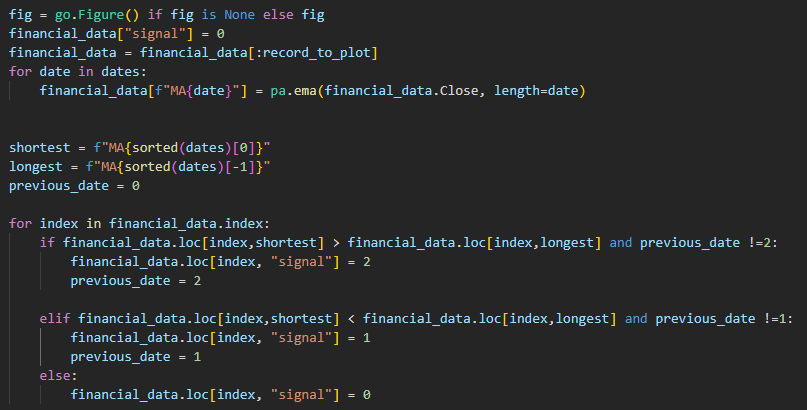
\includegraphics[width=0.8\textwidth]{moving_averages_code.png}
				\caption{Moving Averages}
				\label{fig:moving_averages}

			\end{figure}

			As we can see from the code above, there is a list of numbers that is used to represent the windows that moving averages are going to be calculated on. 
			By using a loop like this I am giving the user the potential to use as many moving averages as they want. However in my implementation I am only using 2 moving averages.
			After successfully writing them down into my data frame I am detecting the shortest and longest as they are then going to be used to detect the crossovers and crossunders.
			After successfully detecting the shortest and longest moving averages I am than checking for potential crossovers and crossunders. Once again
			I am using the strategy that if the previous signal was a buy I am only looking for a sell signal and vice versa. This is done in order to prevent the strategy from just hoarding 
			buy and sell signals and not being able to detect the trend changes. The strategy of hoarding buys works however in this research I am looking inside of
			a trading strategy, not investing strategy.
			\subsubsection{Trend detection}
				Bullish trend is signaled when the shortest moving average is higher than the longest moving average and the previous signal was a sell.
				Bearish trend is signaled when the shortest moving average is lower than the longest moving average and the previous signal was a buy.

			\subsubsection{Performance}
				\begin{figure}[h!]
					\centering
					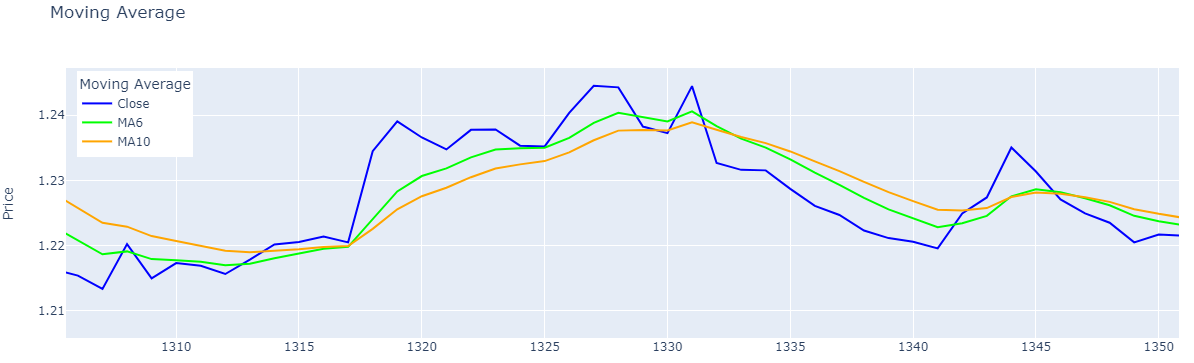
\includegraphics[width=0.8\textwidth]{moving_averages_plot.png}
					\caption{Moving Averages Performance}
					\label{fig:moving_averages_performance}
				\end{figure}
				On this plot we can see 3 lines with the following colors: Blue, Orange and Green. The blue line is the close price of the market, the orange line is the moving average for 
				a window of 10 periods and the green line is the moving average for a window of 6 periods. 
				In certain occasions the green line (MA6) is above the orange line (MA10) and in certain occasions the orange line (MA10) is above the green line (MA6).
				When the green line (MA6) is above the orange line (MA10) we are in a bullish trend and when the orange line (MA10) is above the green line (MA6) we are in a bearish trend.
				Moving Averages seem to be the best performing Technical Indicator so far. It was able to detect trend changes exceptionally well and was able 
				to capitalize on the trend reversals exceptionally. Even though the strategy is very volatile as I have set the windows to be very short term it performed 
				very well and was able to generate a very high return on investment.
				The metrics of the Moving Averages are the following:
				\begin{table}[h!]
					\centering
					\begin{tabular}{|c|c|c|c|c|}
						\hline
						\textbf{ROI} & \textbf{Win Rate} & \textbf{Buy \& Hold Return} & \textbf{Average Trade Return} \\ \hline
						26.1\%         & 69.2\%               & 8.8\%                         & 1.6\%                           \\ \hline
					\end{tabular}
					\caption{Moving Averages Performance Metrics}
					\label{tab:moving_averages_performance_metrics}
				
				\end{table}
				Overall performance of Moving Averages are astonishing as it was able to generate a return on investment of 26.1\%. However it is important to look at the following 
				metric: Win Rate. The win rate of Moving Averages is 69.2\% which is very low compared to the previous Technical Indicators. This is due to the fact that the strategy I have 
				chosen is very volatile. Even though the average trade return is 1.6\% which is also very low compared to the previous Technical Indicators. This is also due to the small size 
				of windows I have chosen. If the windows would have been larger it would take longer time to detect the trend reversals.
	

\chapter{Conclusion}

	The goal of this research was to determine whether Technical Indicators and Machine learning strategies are a viable option for time series forecasting. In this section I am going to answer 
	the research question and summarize the results of the research.
	\section{Machine Learning Strategies}
		Out of the 4 Machine Learning strategies 
		I have tested all of them were able to get decent results in terms of the metrics. The strategies were the following: LSTM Neural Network, ARIMA and XGBoost. The 4th strategy which was SVR was 
		not as successful as the other 3.
		The research question was the following:
		\subsubsection{
			What is the comparative performance and predictive accuracy of a machine learning
			algorithms and technical indicators for price forecasting in financial markets?
			} 


		Overall average metrics achieved are the following:
		\begin{table}[h!]
			\centering
			\begin{tabular}{|c|c|c|c|c|}
					\hline
					\textbf{Strategy} &		\textbf{MAE} & \textbf{MSE} & \textbf{RMSE} & \textbf{R2} \\ \hline
					LSTM             				 & 0.0 & 0.012 & 0.014 & 0.029  \\ \hline
					ARIMA            				 & 0.002 & 8.489e-06  & 0.003 & 0.952 \\ \hline
					XGBoost      	 				 &  0.068 & 0.098 &  0.089 &  0.50 \\ \hline
					SVR        		 				 & 0.263 & 0.297 & 0.371 & -0.483 \\ \hline
				
			\end{tabular}
			\caption{Machine Learning Strategies Metrics}
			\label{tab:machine_learning_strategies_metrics}
		\end{table}

		Out of all the Models we can see that ARIMA is the best performing model in terms of the metrics. All of the models have a relativelt low MAE and MSE which is a good sign. The second best performing model is LSTM which is a Neural Network.
		By enabling larger model with up to 64 neurons and 5 layers and one output one I was able to achieve a very low metrics overall. The third best performing model is XGBoost which is a Gradient Boosting model. This model is very good at detecting trends.
		Its metrics are still amazing however in comparison to the other 2 models it is not as good. The worst performing model is SVR which is a Support Vector Machine model. This model is not as good at detecting trends and is not as good at predicting the future.
		The negative R2 score is a clear indicator of that. However the model is still able to achieve a relatively low MAE and MSE which is a good sign. RMSE of 0.371 is not the best however it is still relatively low.
		\subsubsection{Is it possible to predict the future price of the stock market based on historical data?}
			Yes, the first 3 models are able to do so with a very low error rate all over the board. 
			Is it possible to predict the future price of the stock market based on historical data using SVR? Yes, however the error rate is higher than the other 3 models.
	
	\section{Technical Indicators}
		From the 4 technical indicators I have tested all of them were able to get great results and achieve a very high return on investment. The 4 technical indicators were the following: RSI, Bollinger Bands, Rolling Windows and Moving Averages.
		The research question was the following:
		\subsubsection{
			What is the comparative performance and predictive accuracy of a machine learning
			algorithms and technical indicators for price forecasting in financial markets?
			}
		Overall average metrics achieved are the following:
		\begin{table}[h!]
			\centering
			\begin{tabular}{|c|c|c|c|c|}
					\hline
					\textbf{Strategy} &		\textbf{ROI} & \textbf{Win Rate} & \textbf{Buy \& Hold Return} & \textbf{Average Trade Return} \\ \hline
					RSI             				 & 17.4\% & 95.7\% & 10.6\% & 2.5\%  \\ \hline
					Bollinger Bands            				 & 20.5\% & 92.6\%  & 5.5\% & 2.4\% \\ \hline
					Rolling Windows      	 				 &  20.0\% & 90.5\% & 10.6\% & 2.8\% \\ \hline
					Moving Averages        		 				 & 26.1\% & 69.2\% & 8.8\% & 1.6\% \\ \hline
			\end{tabular}
			\caption{Technical Indicators Metrics}
			\label{tab:technical_indicators_metrics}
		\end{table}

		All of the models have an exceptionally high return on investment for a financial market like the currency exchange one. The best performing model is Moving Averages with a return on investment of 26.1\%.
		The second best performing model is a Bollinger Bands with a return on investment of 20.5\%. with a buy and hold return of 5.5\%. This means the clean profit of the Bollinger Bands is 15\%.
		If the question is to trade safest with a relatively low risk and a high return on investment than the best option would be RSI. the return on investment of RSI is 17.4\% and the win rate is 95.7\%.
		The win rate of 95.7\% is exceptionally high and is a clear indicator for a safe trading strategy. 
		\subsubsection{Is it possible to predict the future price of the stock market based on historical data?}
			Yes, all of the models are able to outperform the market and are able to generate a clean profit. Every single one of the models is able to generate a high return on investment in such a stable trading pair like the EUR/GBP one. 
			I am exceptionally satisfied with the results of the research and I believe that the results are very promising. 
			The equity graph can be seen in the following figure:
			
			\begin{figure}[h!]
				\centering

				\begin{subfigure}{0.45\textwidth}
					\centering
					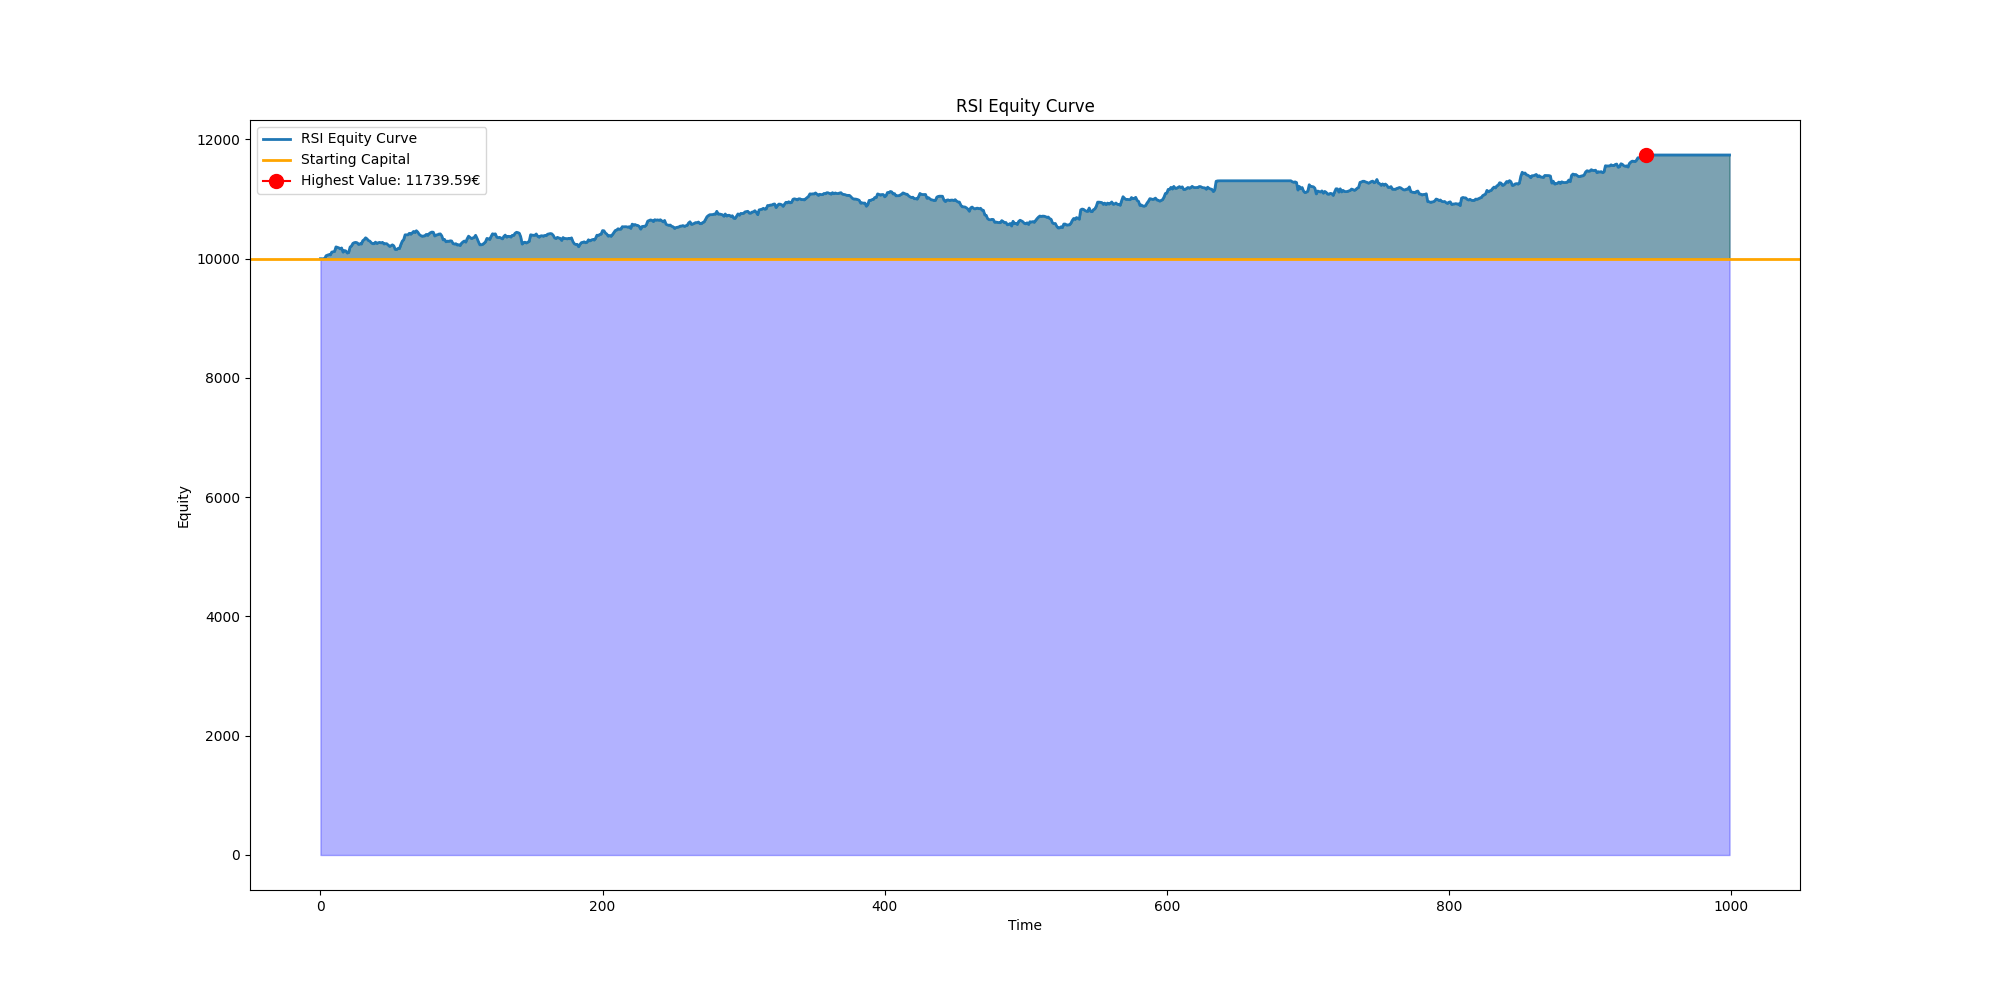
\includegraphics[width=\textwidth]{equity_curve_rsi.png}
					\caption{Equity Curve for RSI}
					\label{fig:equity_curve_rsi}
				\end{subfigure}
				\hfill
				\begin{subfigure}{0.45\textwidth}
					\centering
					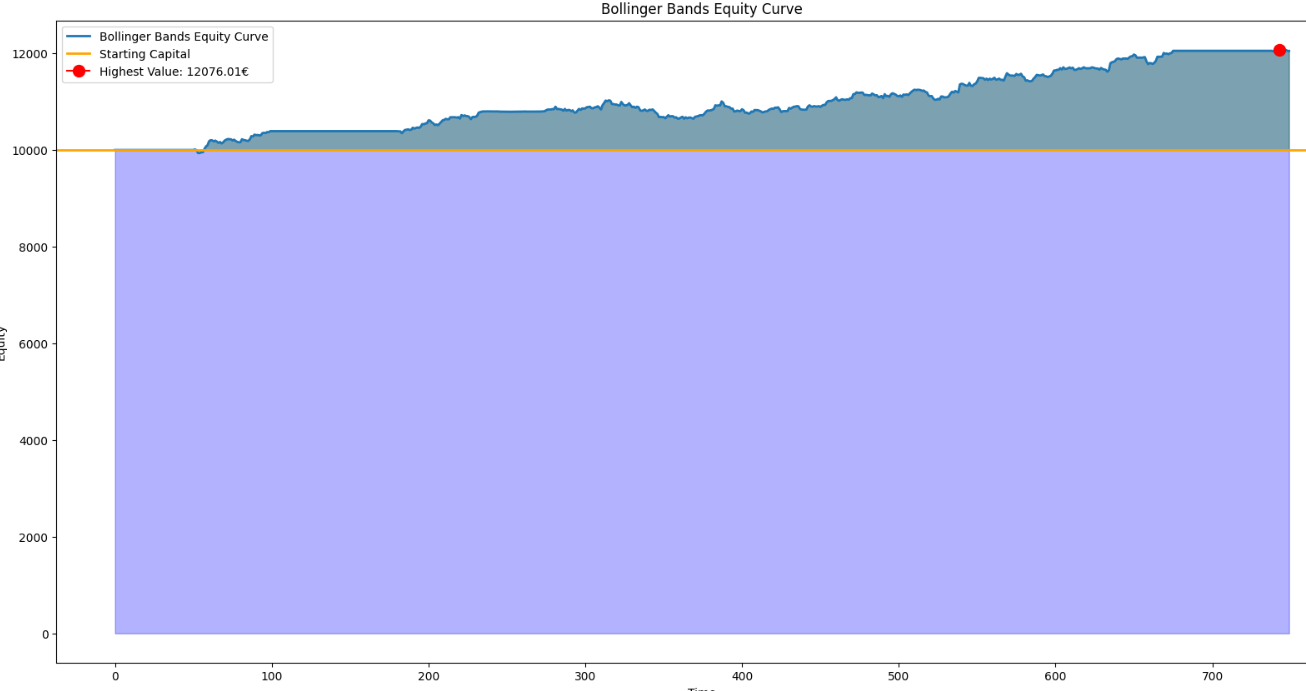
\includegraphics[width=\textwidth]{equity_curve_bollinger_bands.png}
					\caption{Equity Curve for Bollinger Bands}
					\label{fig:equity_curve_bollinger_bands}
				\end{subfigure}

				\begin{subfigure}{0.45\textwidth}
					\centering
					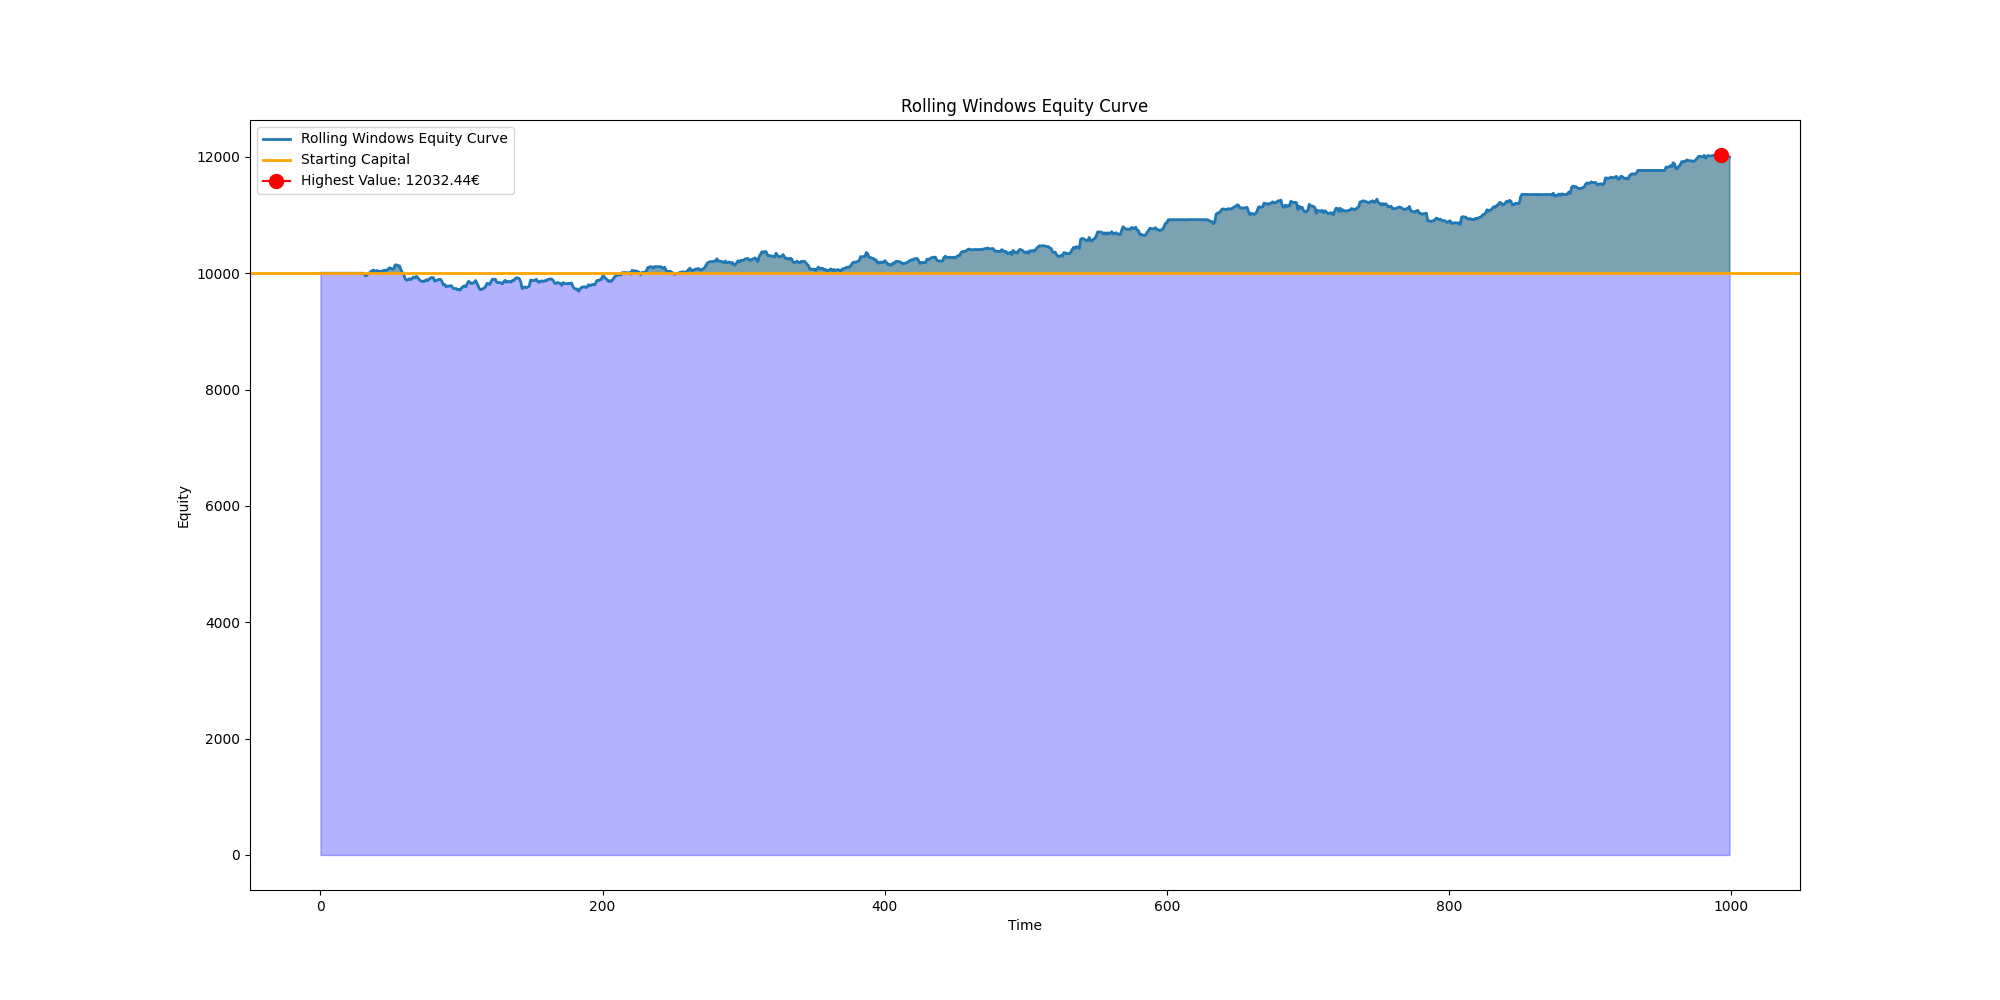
\includegraphics[width=\textwidth]{equity_curve_rolling_windows.png}
					\caption{Equity Curve for Rolling Windows}
					\label{fig:equity_curve_rolling_windows}
				\end{subfigure}
				\hfill
				\begin{subfigure}{0.45\textwidth}
					\centering
					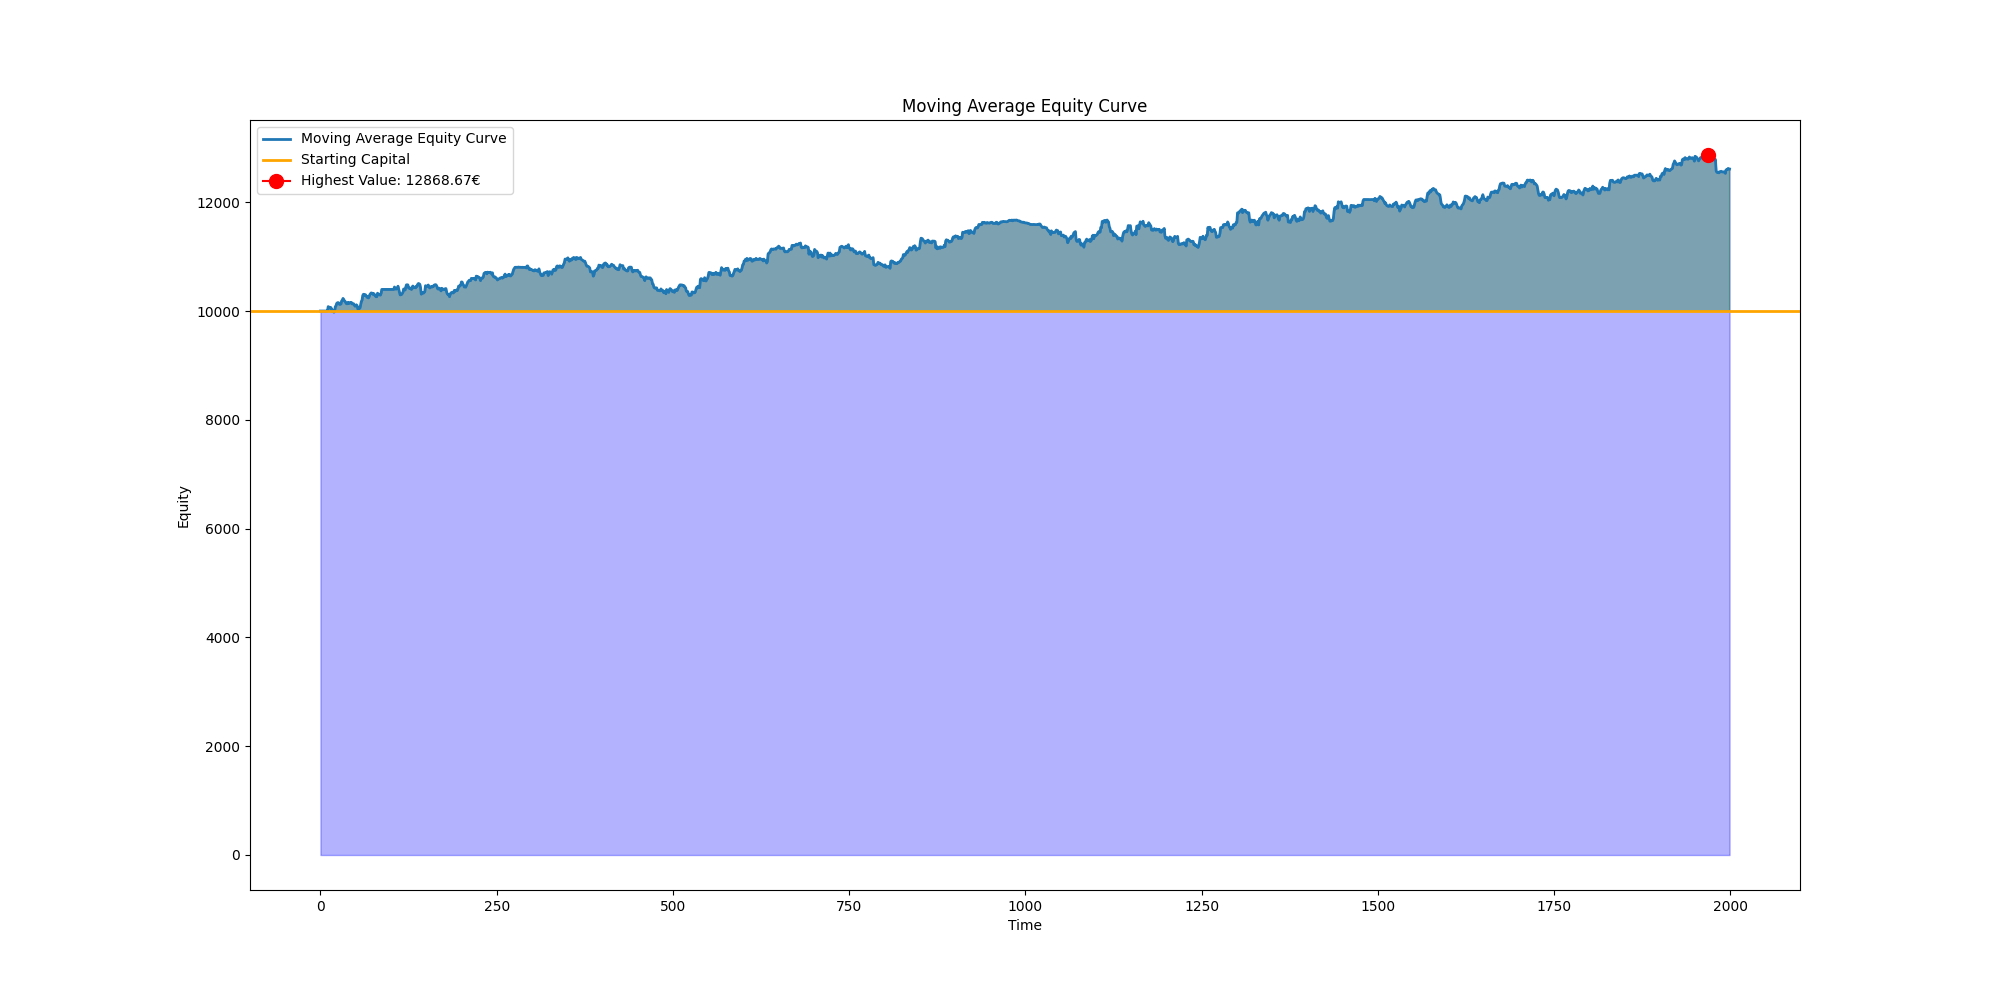
\includegraphics[width=\textwidth]{equity_curve_moving_averages.png}
					\caption{Equity Curve for Moving Averages}
					\label{fig:equity_curve_moving_averages}
				\end{subfigure}

				\caption{Equity Curves for Different Strategies}
				\label{fig:combined_equity_curves}
			\end{figure}
		
	\section{Conclusion}
	During this research I have been exploring the performance of Machine Learning Models and Technical Indicators and studying their performance against each other. I have been using the EUR/GBP currency pair as it is a very stable currency pair.
	Even though the currency pair is very stable and the market could be considered as low volatile, it is important to note that this research could be applied to any other currency pair or even stock market.
	The reason for selecting the specific models and indicators was due to the fact that I wanted to explore the performance of the most popular models and indicators on market with low perecentage differentials.
	There was no initial bias towards any of the model or indicator and nothing has been cherry picked. As I have mentioned before the goal of this research was to determine whether Machine Learning Models 
	and Technical Indicators are a viable option for time series forecasting. The results of the research are very promising and the null hypothesis that it is not possible to forecast the market movement using Machine Learning models
	and Technical Indicators can be rejected. The results speak for themselves and I believe that they could be even better if the research was done on a more volatile market.
	



%   BACK MATTER  %%%%%%%%%%%%%%%%%%%%%%%%%%%%%%%%%%%%%%%%%%%%%%%%%%%%%%%%%%%%%%
%
%   References and appendices. Appendices come after the bibliography and
%   should be in the order that they are referred to in the text.
%
%   If you include figures, etc. in an appendix, be sure to use
%
%       \caption[]{...}
%
%   to make sure they are not listed in the List of Figures.
%

\backmatter%
	\addtoToC{Bibliography}
	\bibliographystyle{IEEEtranS}
 \typeout{}
	\bibliography{references}
	

\end{document}